\documentclass[11pt]{article}

% This first part of the file is called the PREAMBLE. It includes
% customizations and command definitions. The preamble is everything
% between \documentclass and \begin{document}.

\usepackage[margin=1in]{geometry}  % set the margins to 1in on all sides
\usepackage{graphicx}              % to include figures
\usepackage{amsmath}               % great math stuff
\usepackage{amsfonts}              % for blackboard bold, etc
\usepackage{amsthm}                % better theorem environments

\usepackage{array}
\usepackage{booktabs}
\usepackage{soul}
\usepackage{mathrsfs}
\usepackage{enumerate}
\usepackage{multicol}
\usepackage[makeroom]{cancel}
\usepackage{xcolor}
\usepackage{tikz}
\usepackage{pdfpages}

% various theorems, numbered by section

\newtheorem{thm}{Theorem}[section]
\newtheorem{lem}[thm]{Lemma}
\newtheorem{prop}[thm]{Proposition}
\newtheorem{cor}[thm]{Corollary}
\newtheorem{conj}[thm]{Conjecture}
\newtheorem{exer}[thm]{Exercise}

\DeclareMathOperator{\id}{id}

\newcommand{\bd}[1]{\mathbf{#1}}  % for bolding symbols
\newcommand{\RR}{\mathbb{R}}      % for Real numbers
\newcommand{\ZZ}{\mathbb{Z}}      % for Integers
\newcommand{\col}[1]{\left[\begin{matrix} #1 \end{matrix} \right]}
\newcommand{\comb}[2]{\binom{#1^2 + #2^2}{#1+#2}}
\newcommand{\overfrac}[2]{\genfrac{}{}{0pt}{}{#1}{#2}}

\everymath{\displaystyle}

\setlength\parindent{0pt}

\usepackage{setspace}

\begin{document}
\begin{multicols}{2}
  \phantom{hello}\vspace{\baselineskip}
  \phantom{hello}\vspace{\baselineskip}
  {\large Assignment 2}\\
  \begin{flushright}
    Mikhail Gaerlan\\
    21 April 2017\\
    STA 243 Lee
  \end{flushright}
\end{multicols}
\vspace{-1.3\baselineskip}

\hrulefill

\section{Simulated Annealing}

The following table shows the results of the simulated annealing algorithm with various parameters. Each stage contains 100 iterations. The algorithm would stop when either the maximum number of 10,000 stages was reached or the probability of replacing a worse solution was less than $10^{-50}$. The blue data represents the path length of the randomly picked $\theta^*\in N(\theta_k)$ where $N(\theta)$ was the neighborhood of $\theta$ where two elements of $\theta$ were swtiched. The pink data represents the path length of $\theta^*$ such that $\theta_{k+1}=\theta^*$, e.g. when $f(\theta^*)-f(\theta_k)<0$. The figures show clearly that as the temperature decreases, the entropy or randomness of the solutions decreases and cools down towards a minimum. The smaller $p$ values and $\tau_1$ values cause the system to cool down faster. The best solutions found are the sequences (A, I, C, E, H, L, J, O, K, M, F, D, G, N, B) and (A, J, O, K, M, F, N, G, D, L, H, B) both with a path length of 17.

\begin{table*}[h]
  \begin{center}
    \renewcommand{\arraystretch}{1.5}
    \begin{tabular}{| >{\centering\arraybackslash}m{0.5in} |  >{\centering\arraybackslash}m{1.75in} |  >{\centering\arraybackslash}m{1.75in} |  >{\centering\arraybackslash}m{1.75in}|}
      \hline
      &$\tau_1=400$&$\tau_1=200$&$\tau_1=100$\\\hline
      $p=0.999$&
      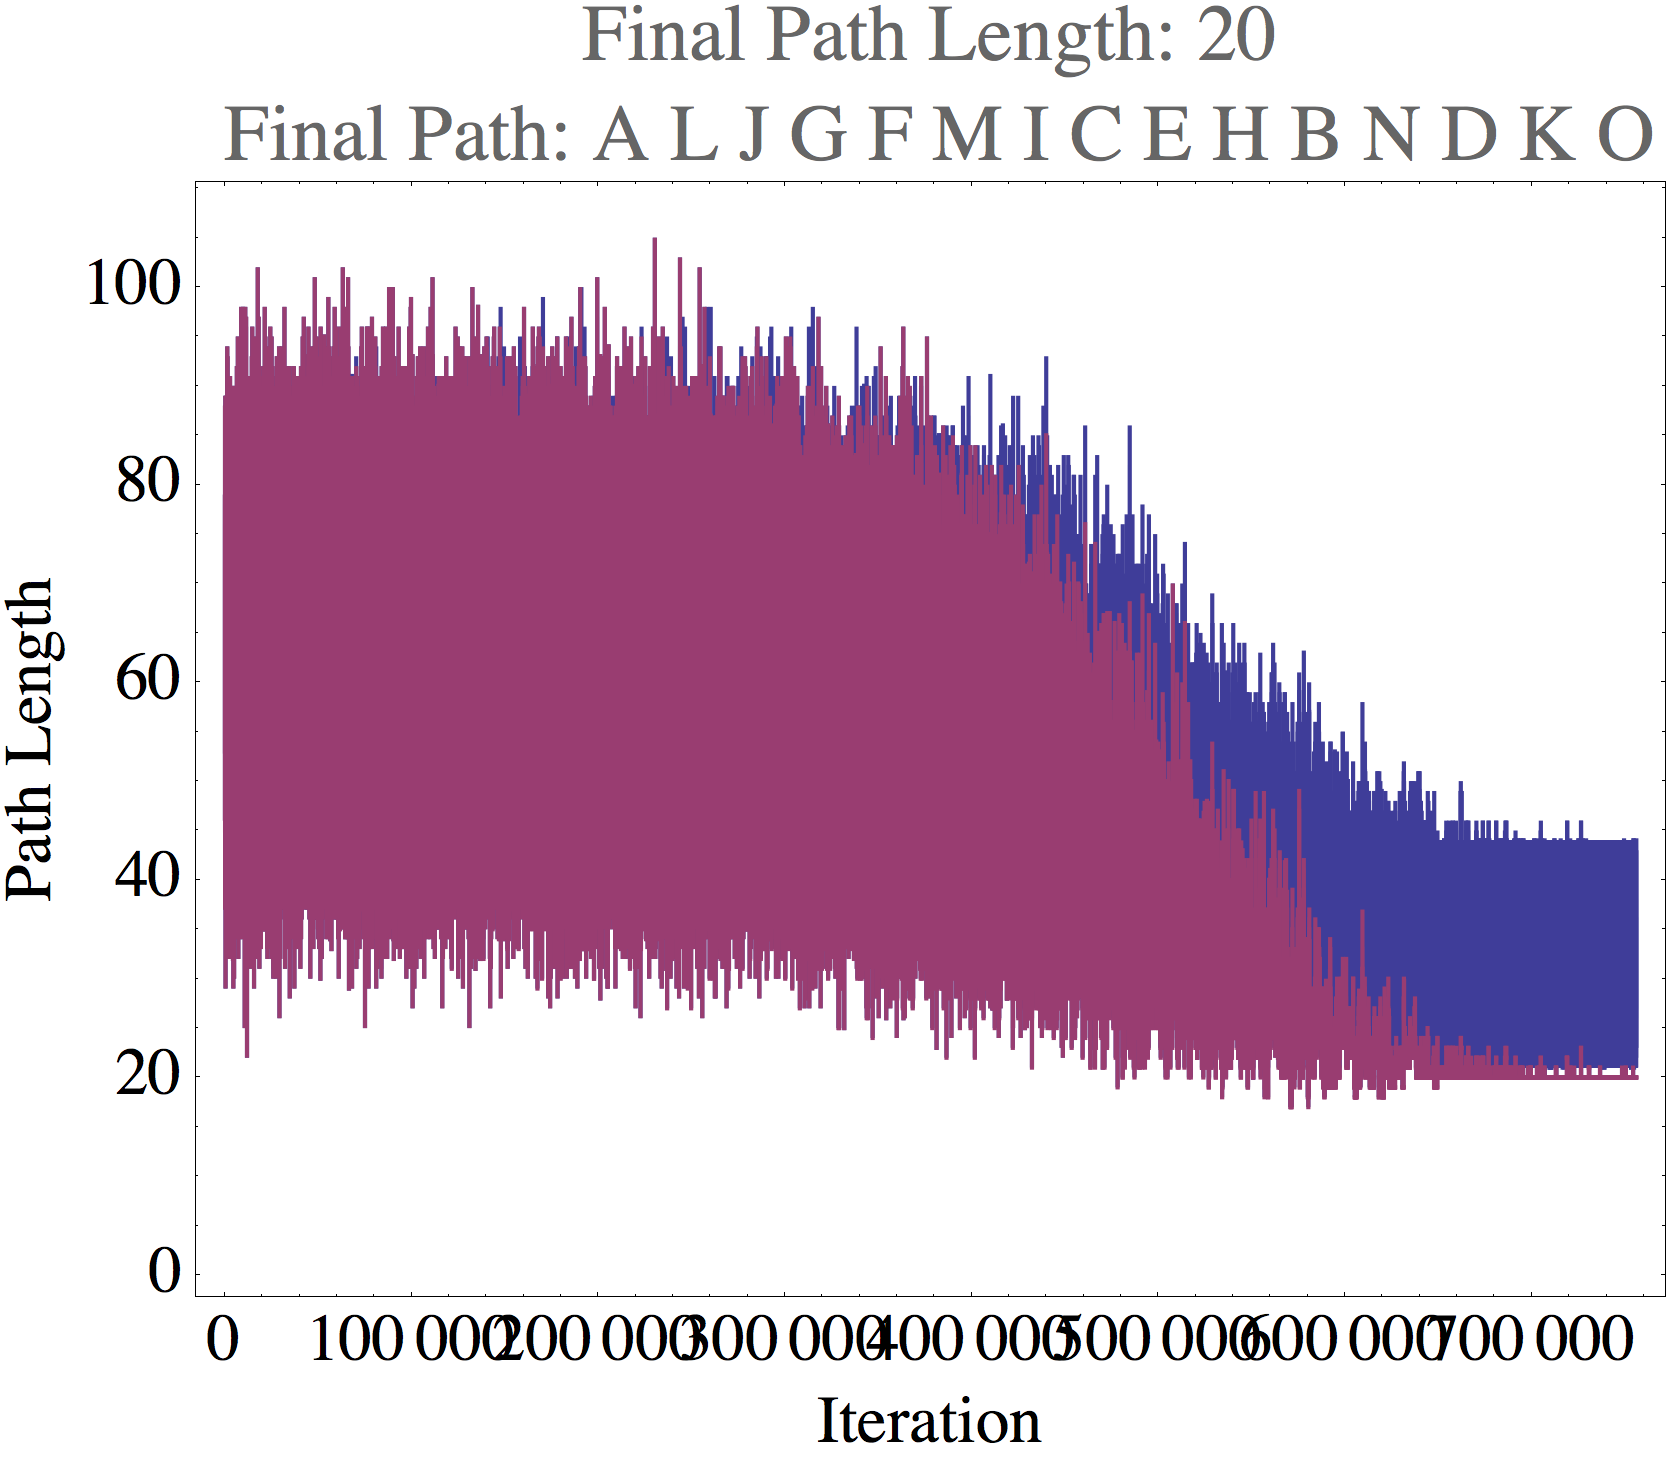
\includegraphics[width=\linewidth,height=0.15\textheight]{resultsp999t400.png}&
      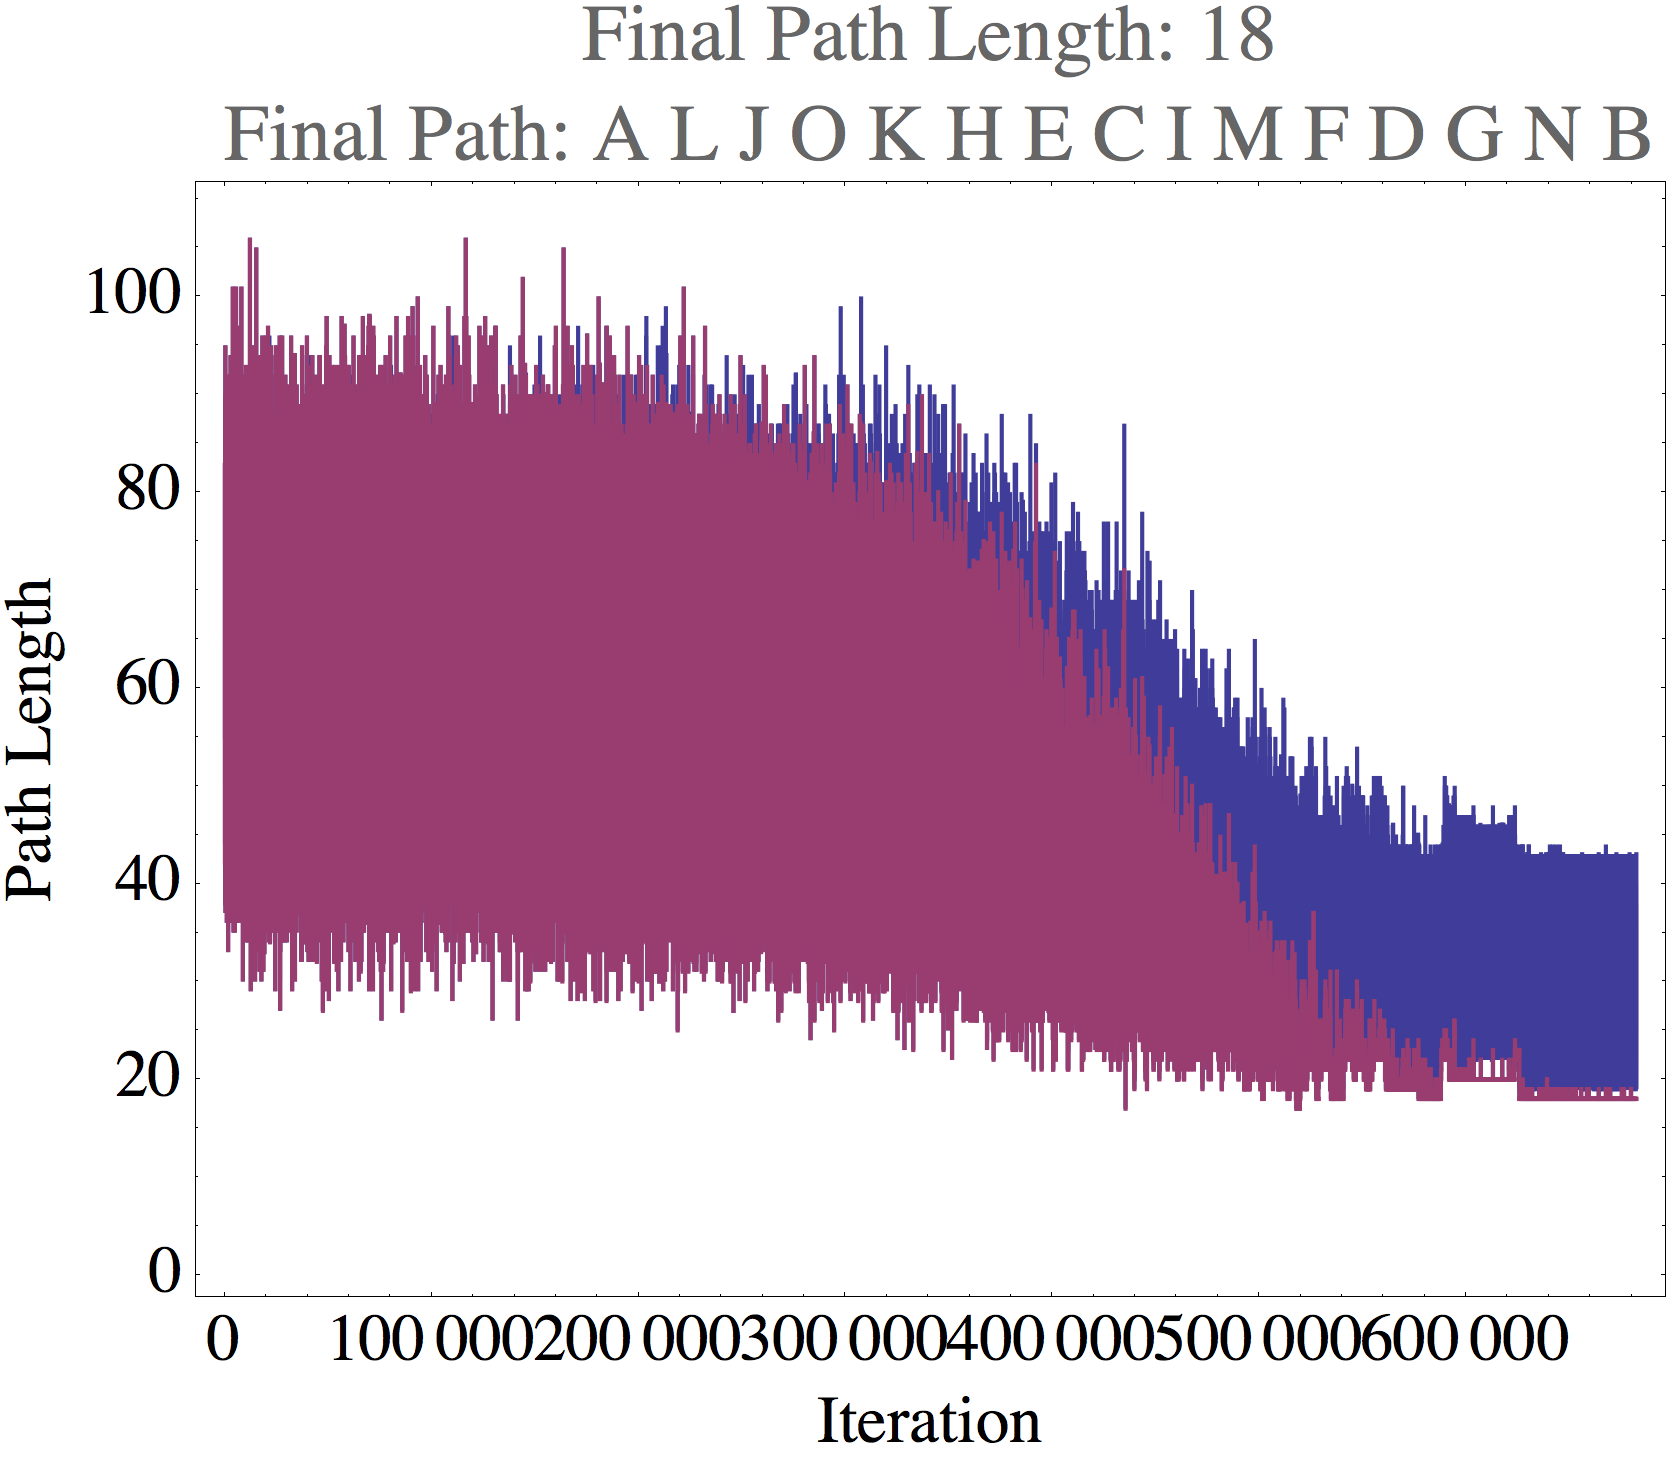
\includegraphics[width=\linewidth,height=0.15\textheight]{resultsp999t200.png}&
      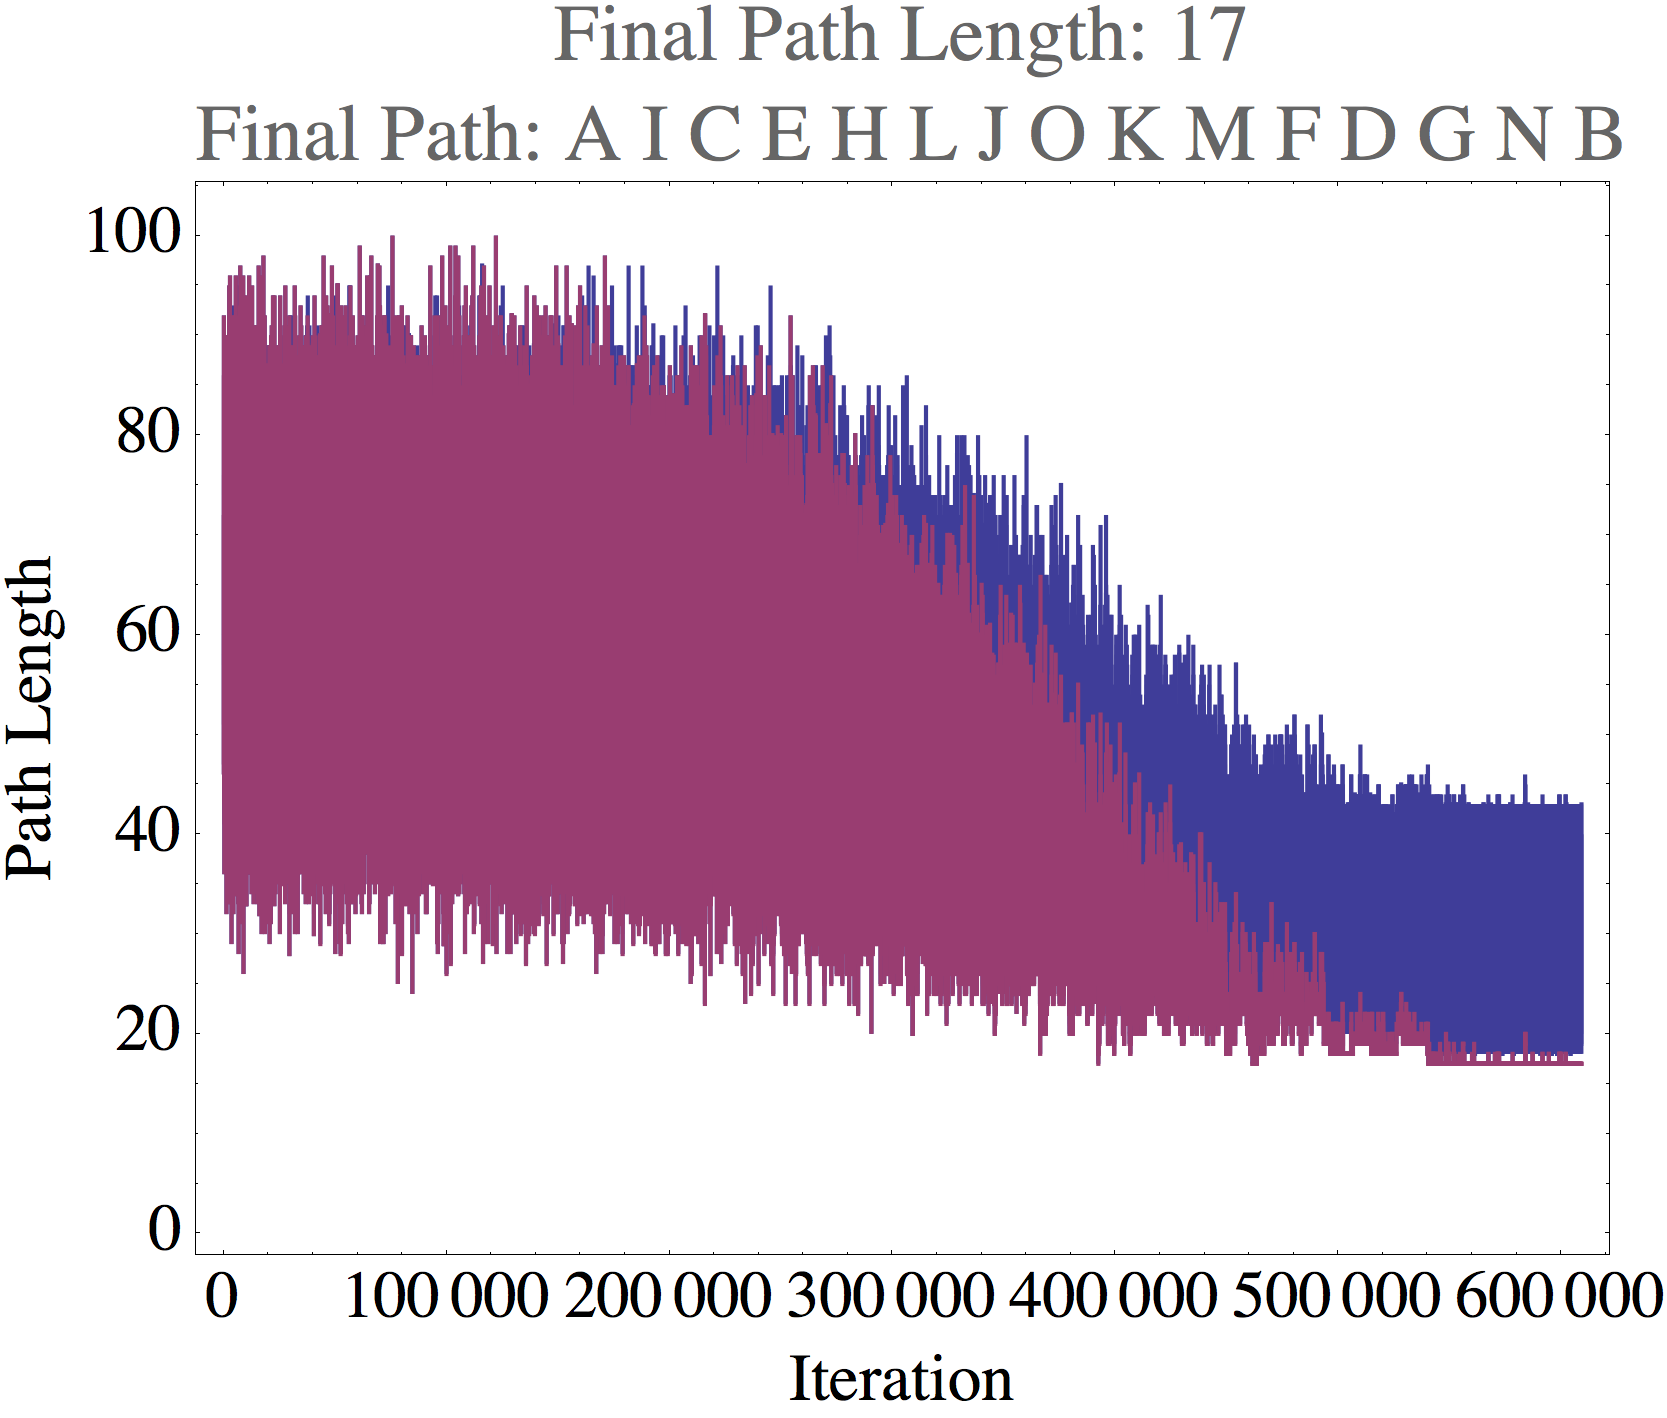
\includegraphics[width=\linewidth,height=0.15\textheight]{resultsp999t100.png}\\\hline
      $p=0.970$&
      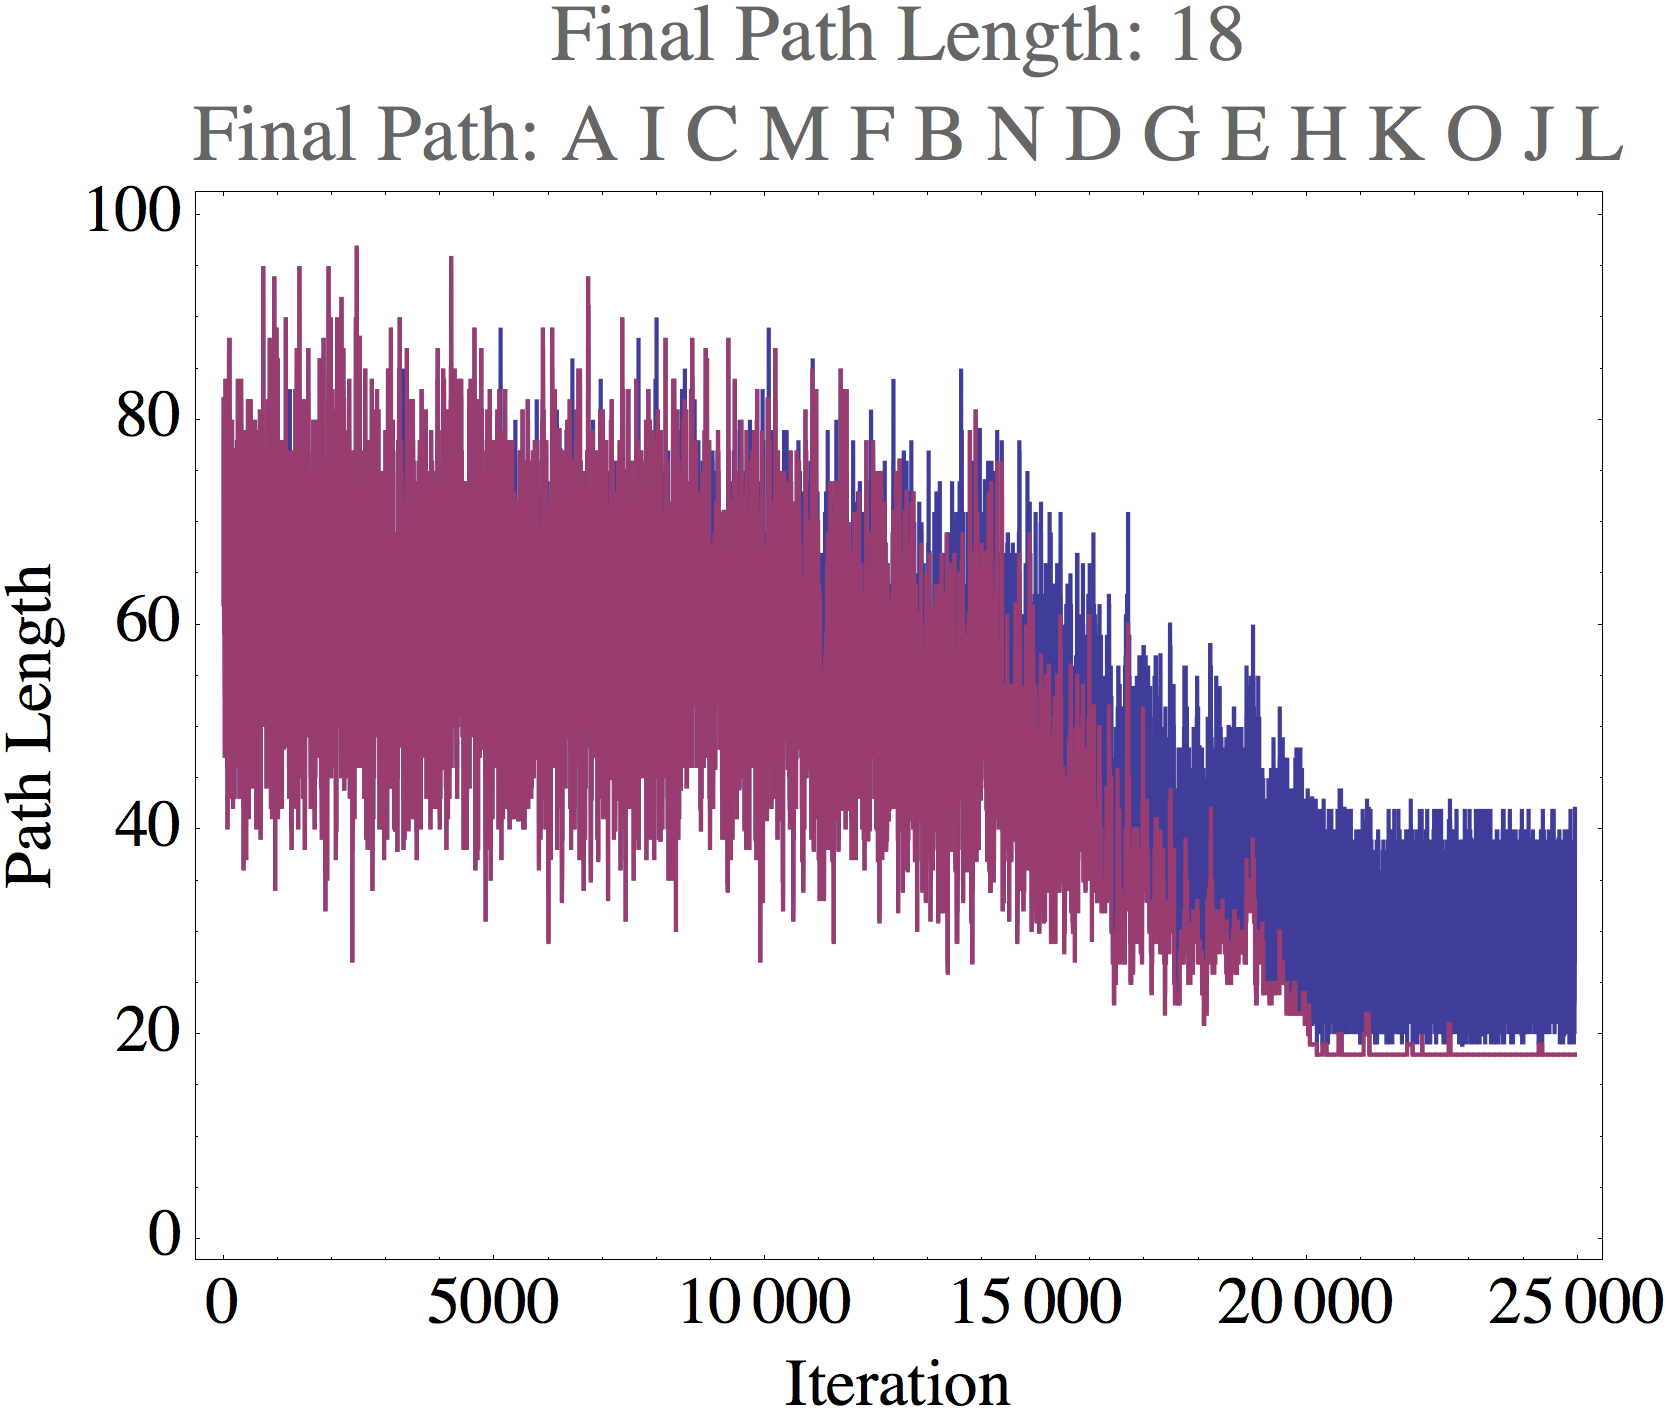
\includegraphics[width=\linewidth,height=0.15\textheight]{resultsp970t400.png}&
      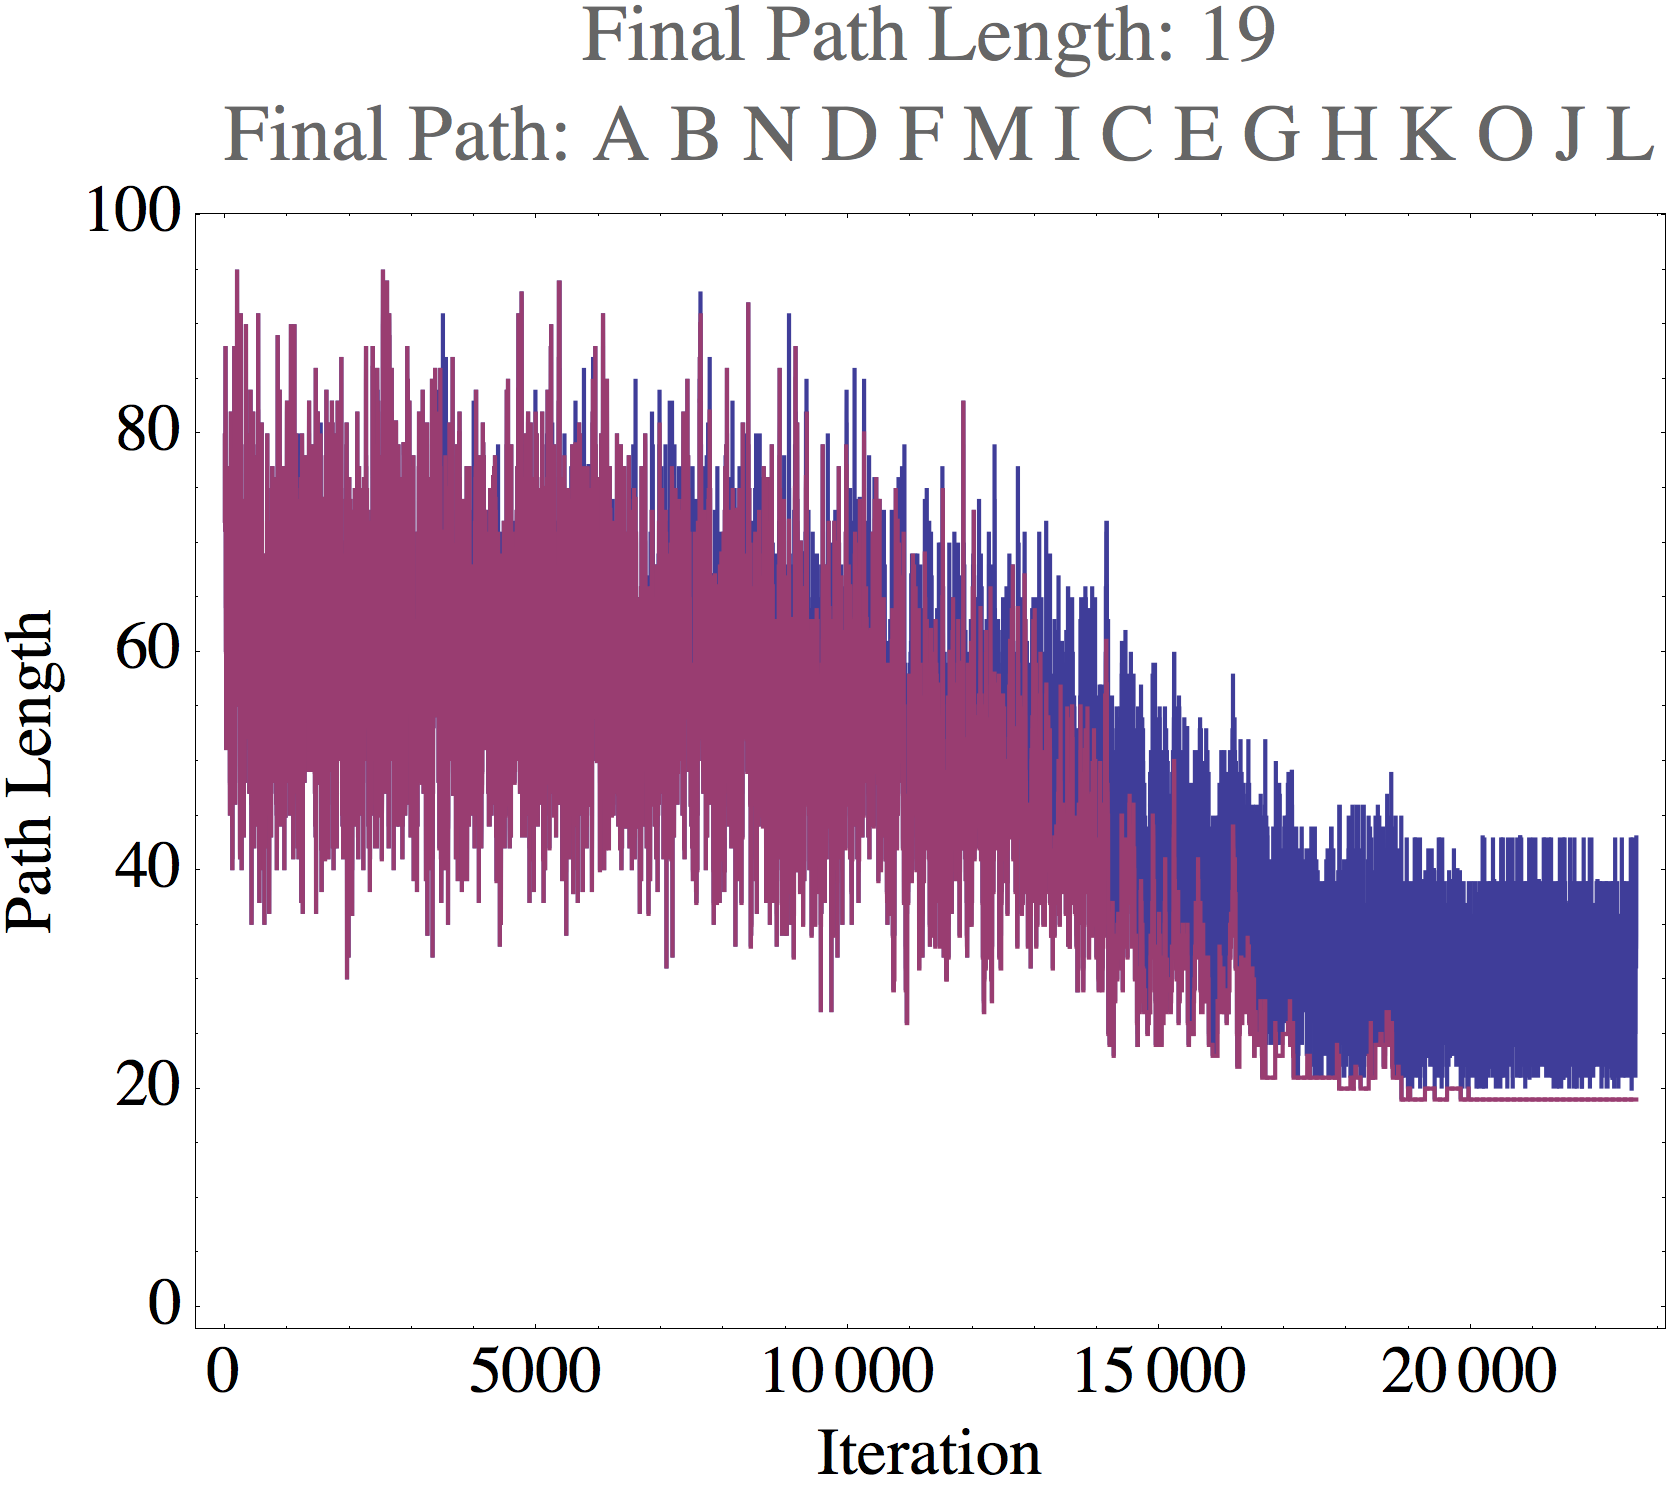
\includegraphics[width=\linewidth,height=0.15\textheight]{resultsp970t200.png}&
      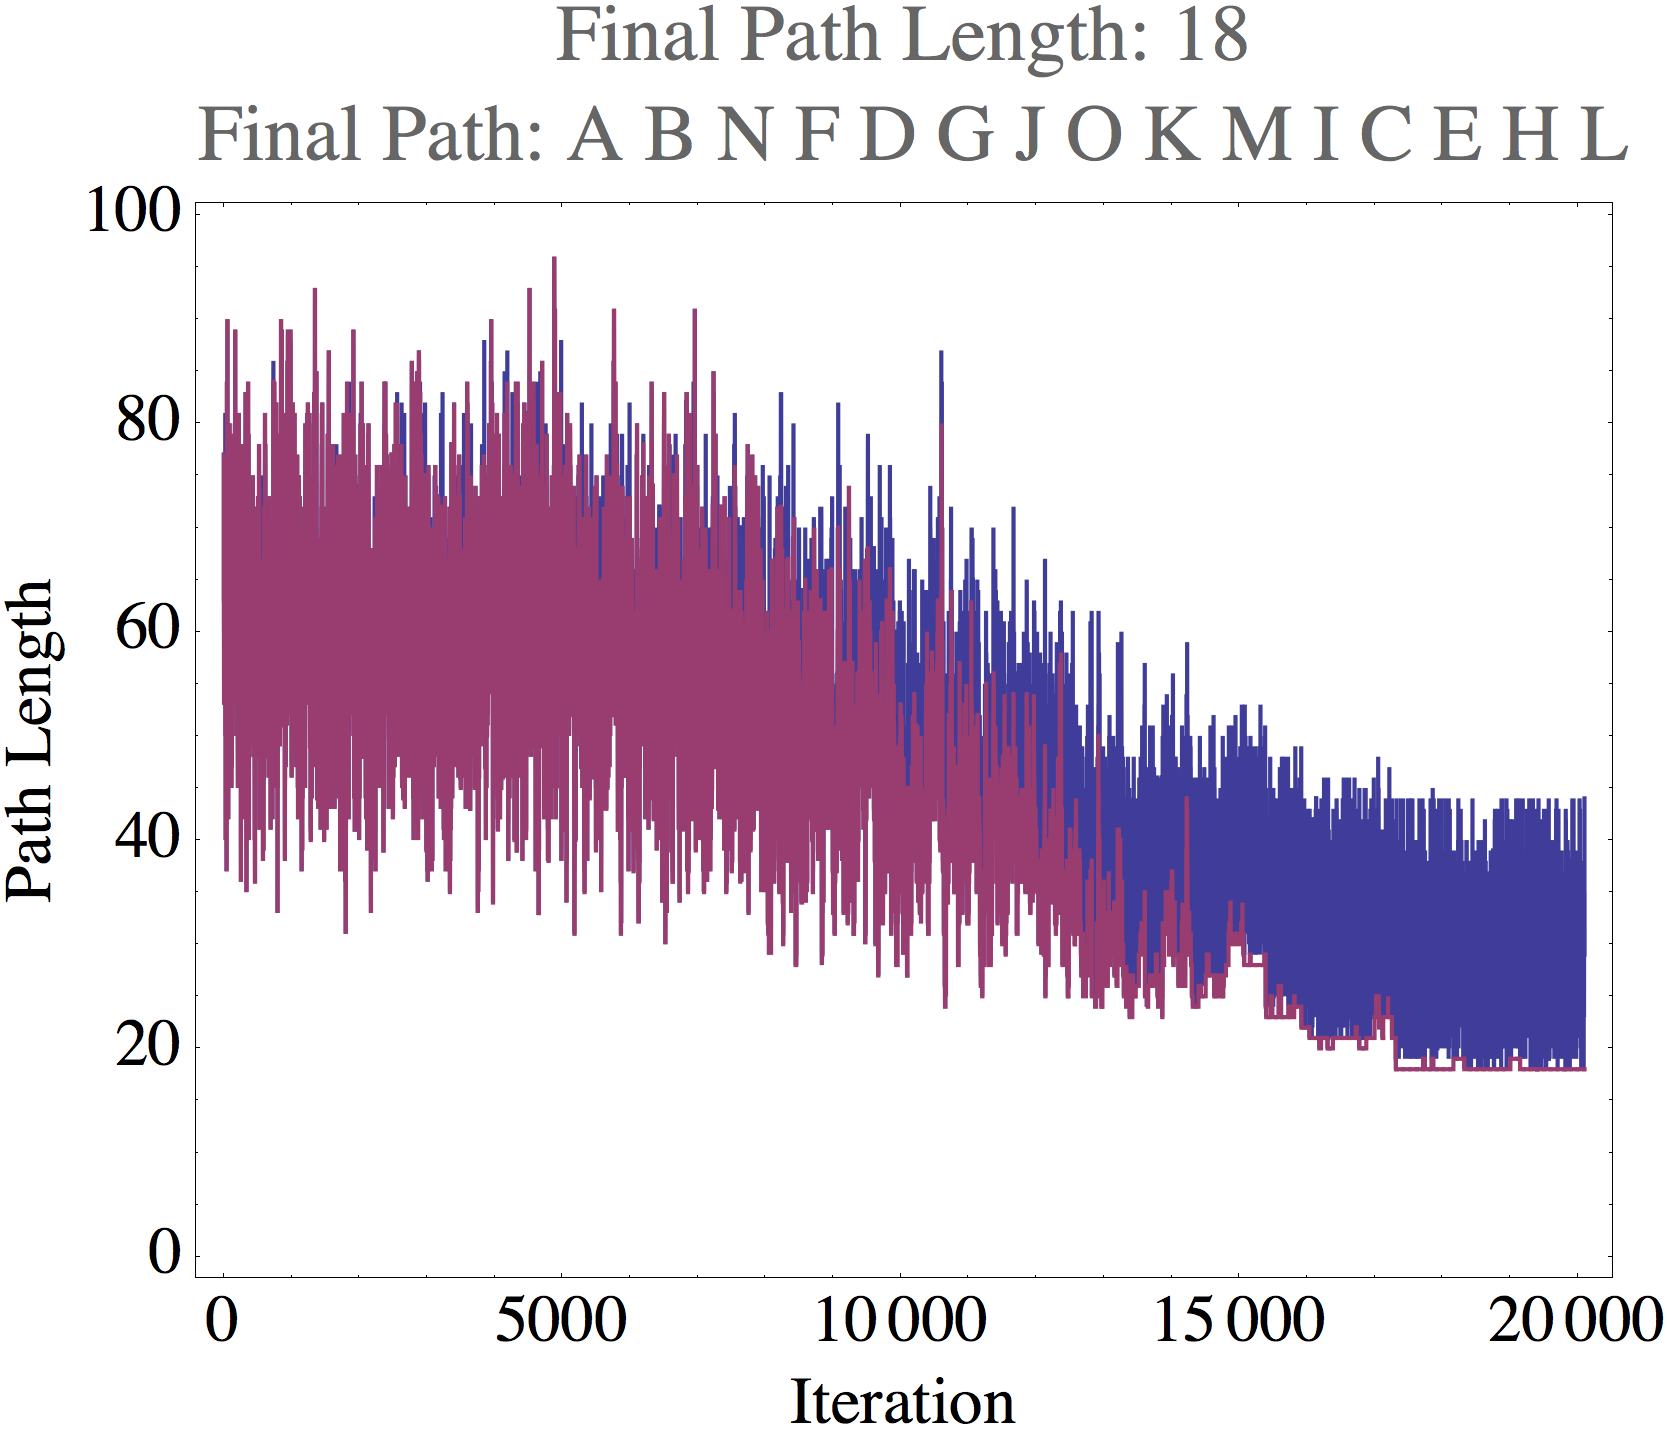
\includegraphics[width=\linewidth,height=0.15\textheight]{resultsp970t100.png}\\\hline
      $p=0.900$&
      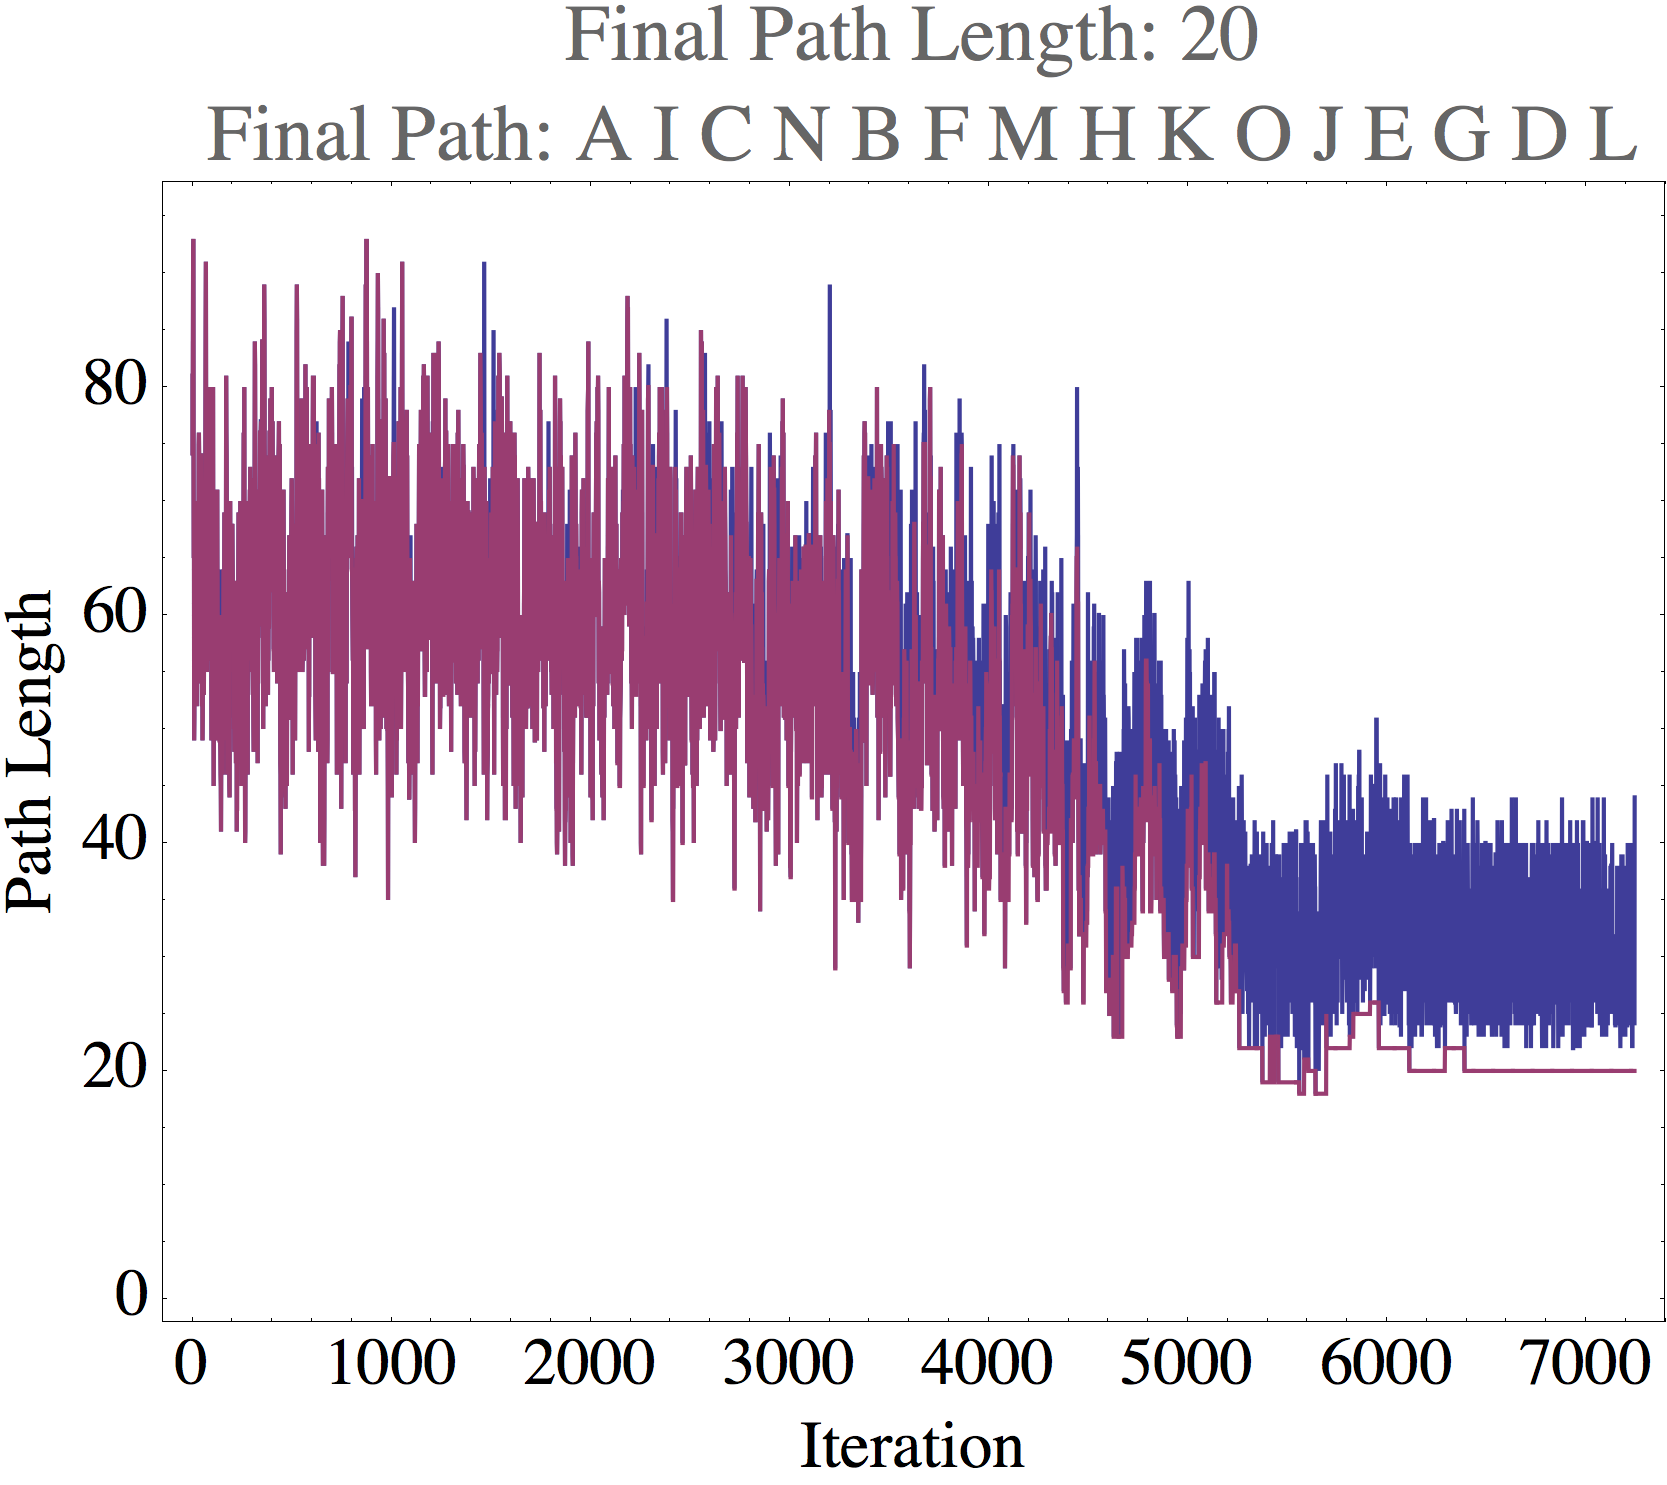
\includegraphics[width=\linewidth,height=0.15\textheight]{resultsp900t400.png}&
      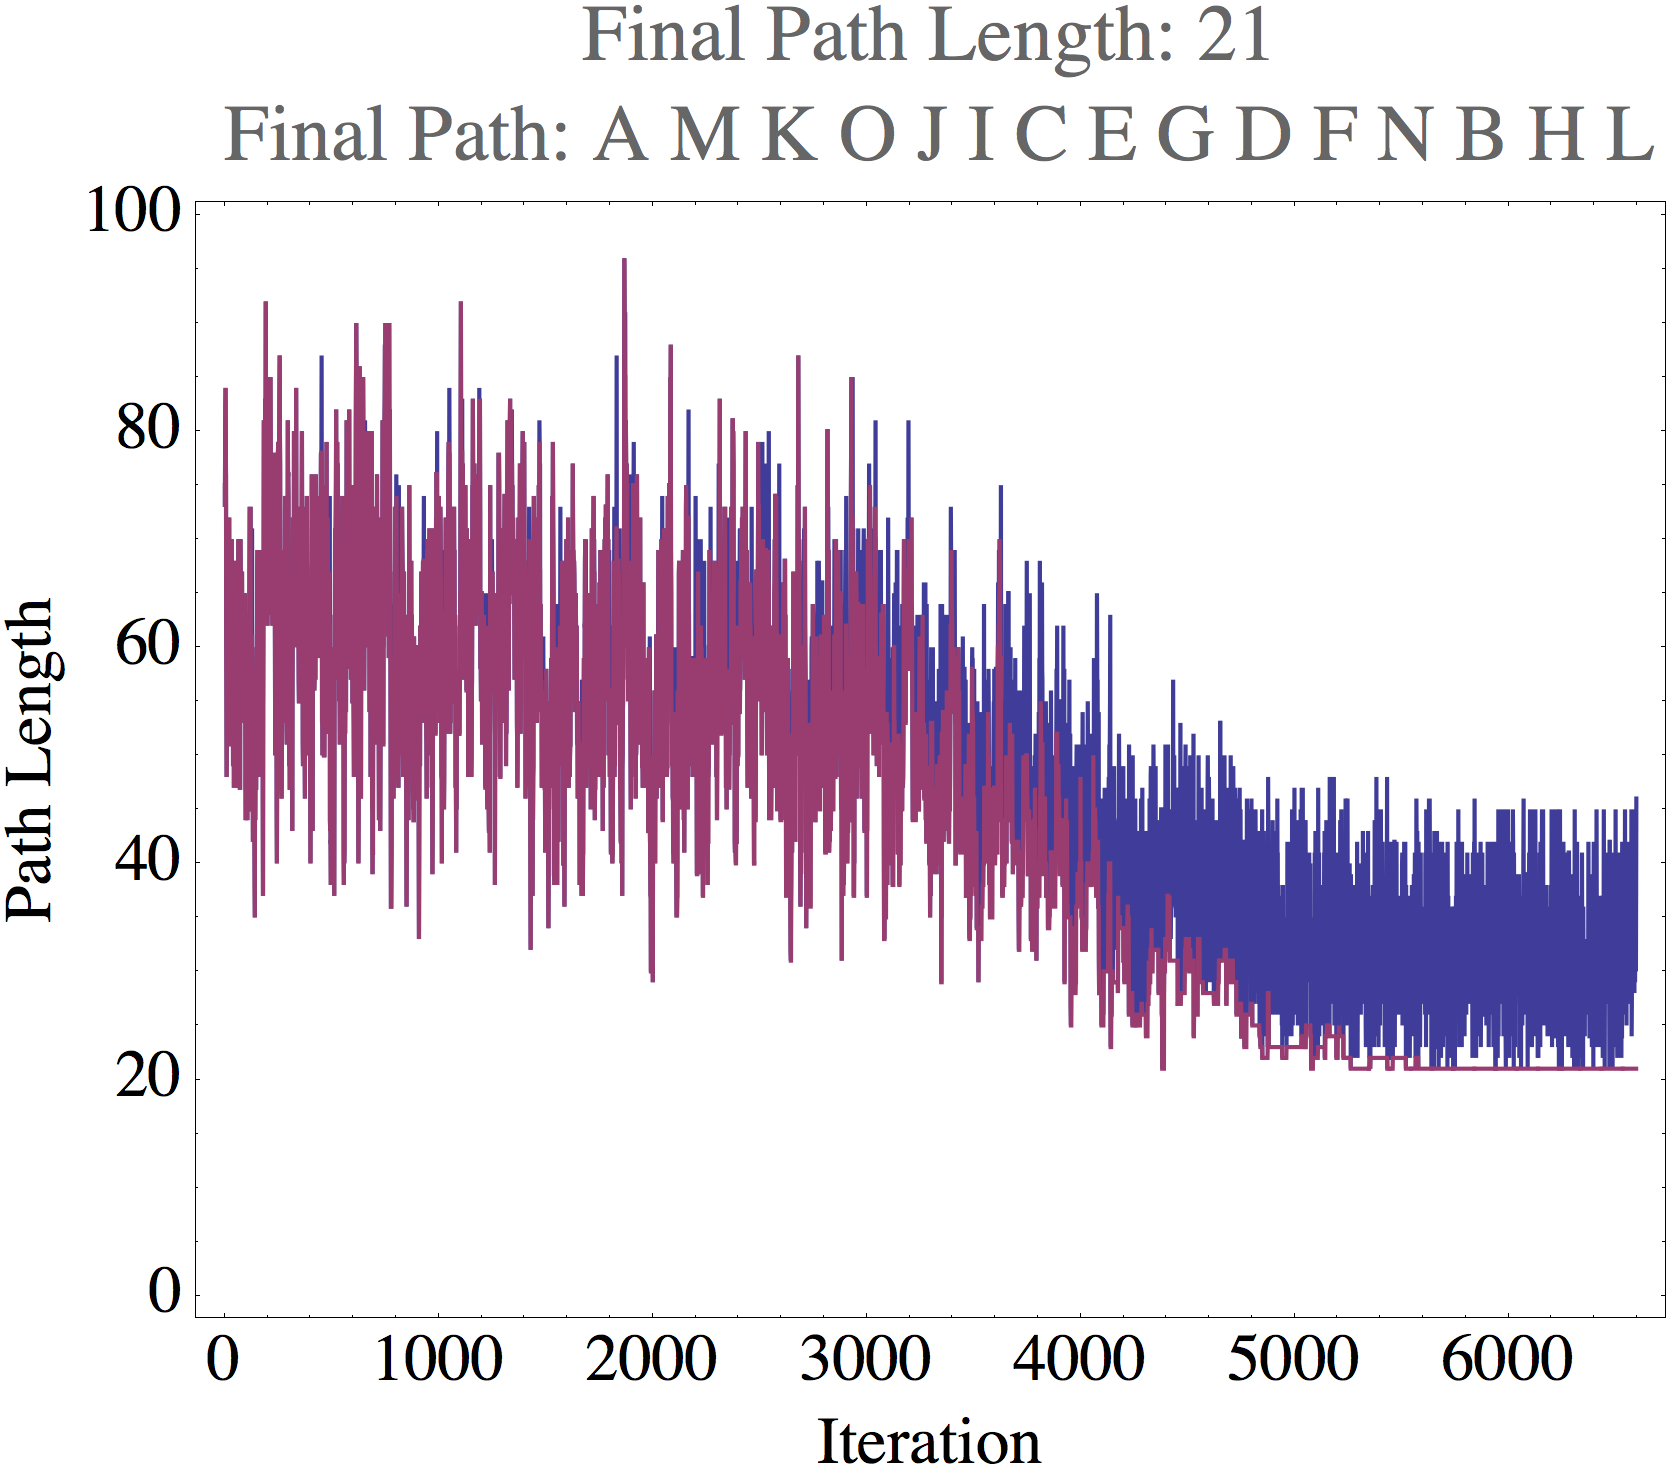
\includegraphics[width=\linewidth,height=0.15\textheight]{resultsp900t200.png}&
      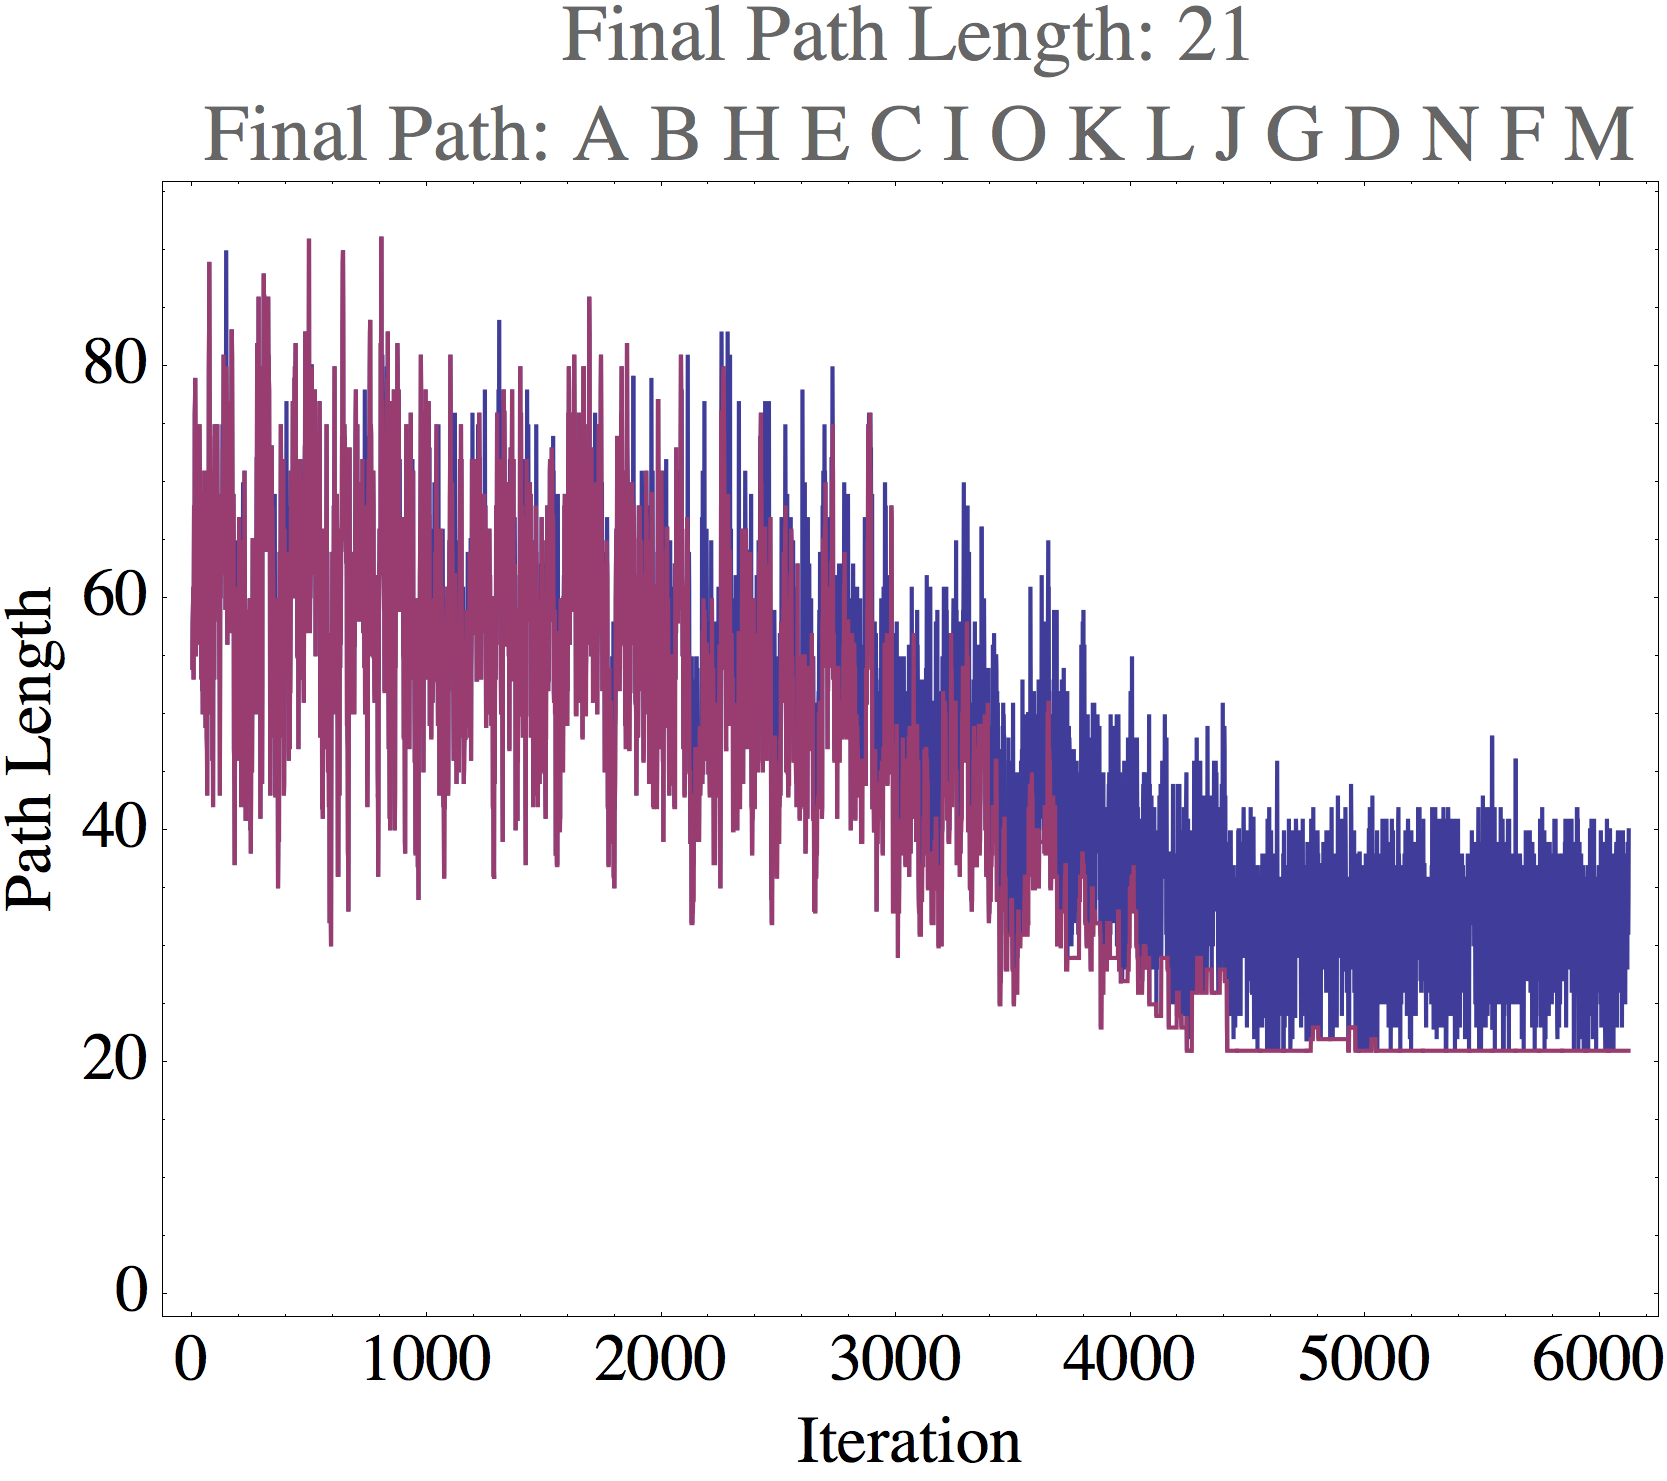
\includegraphics[width=\linewidth,height=0.15\textheight]{resultsp900t100.png}\\\hline
    \end{tabular}
  \end{center}
\end{table*}

\section{Genetic Algorithms}

The initial result for the genetic algorithm is shown in Figure \ref{initial}. While the model appears to fit the data, the data has been over-fit and very noisy as well.

\begin{figure}[h!]
\begin{center}
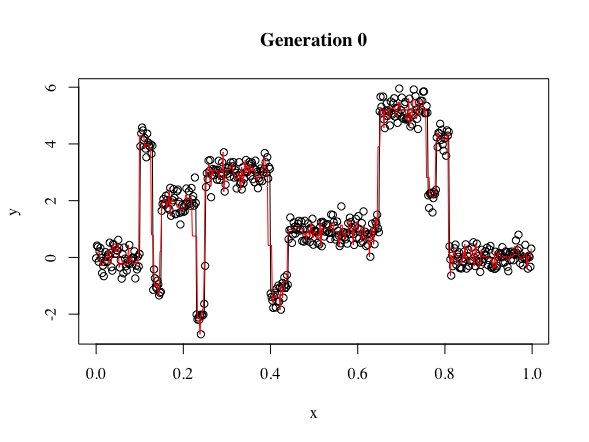
\includegraphics[height=0.3\textheight,width=0.6\linewidth]{initial_gen}
\end{center}
\label{initial}
\end{figure}

The figures in the table on the next page, show the results of the genetic algorithm with different criteria and different algorithm parameters. The algorithm was able to minimize the MDL and AIC. The model achieved getting fewer pieces in the function, but the models found by the algorithm do not seem to fit the data very well.

\begin{table*}[h]
  \begin{center}
    \renewcommand{\arraystretch}{1.5}
    \begin{tabular}{| >{\centering\arraybackslash}m{0.5in} |  >{\centering\arraybackslash}m{2.5in} |  >{\centering\arraybackslash}m{2.5in} | }
      \hline
      &$S=300,N_{\textrm{stop}}=20$&$S=500,N_{\textrm{stop}}=30$\\\hline
      MDL&
      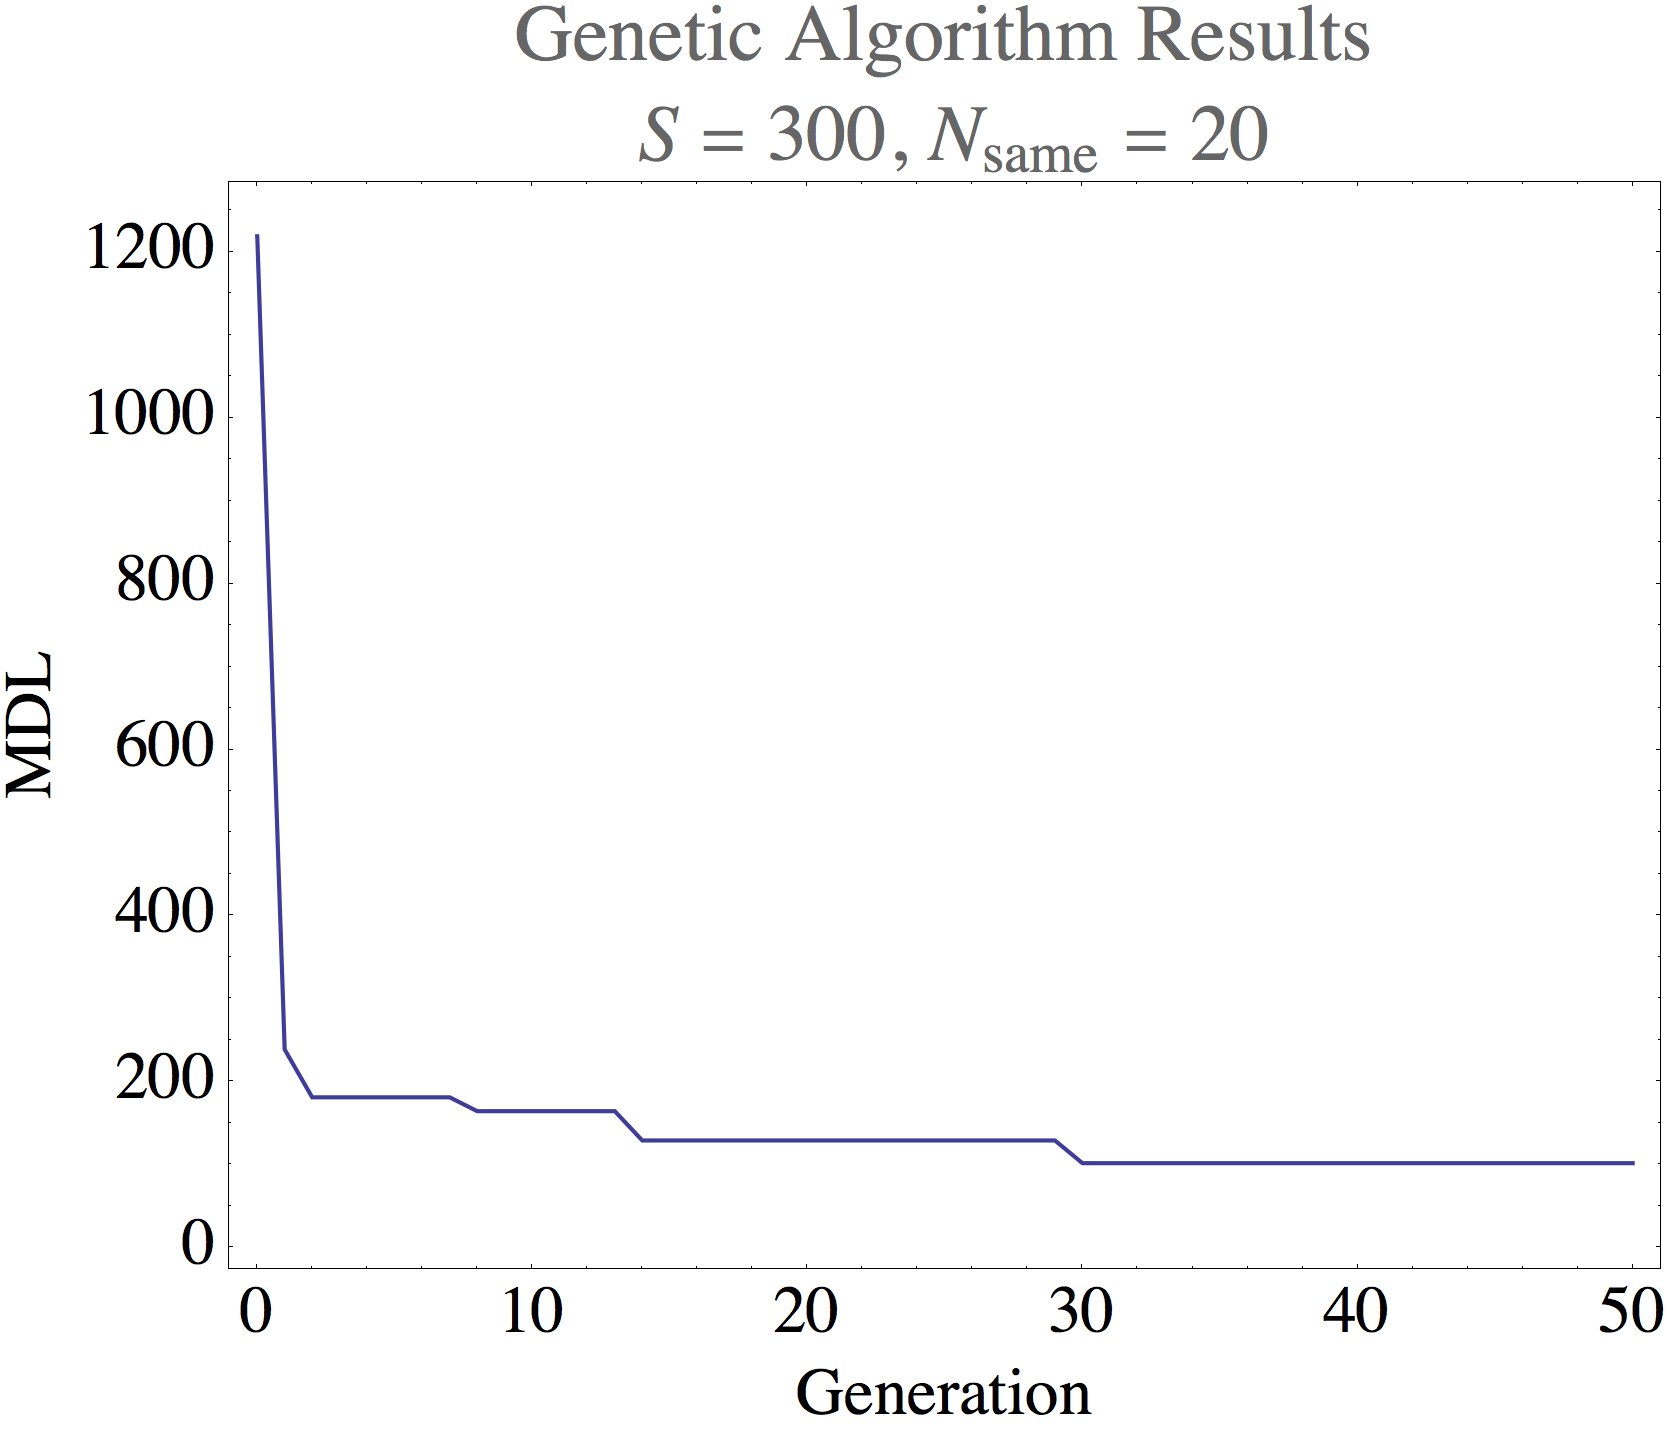
\includegraphics[width=\linewidth,height=0.20\textheight]{mdl_gen_data_300_20.png}&
      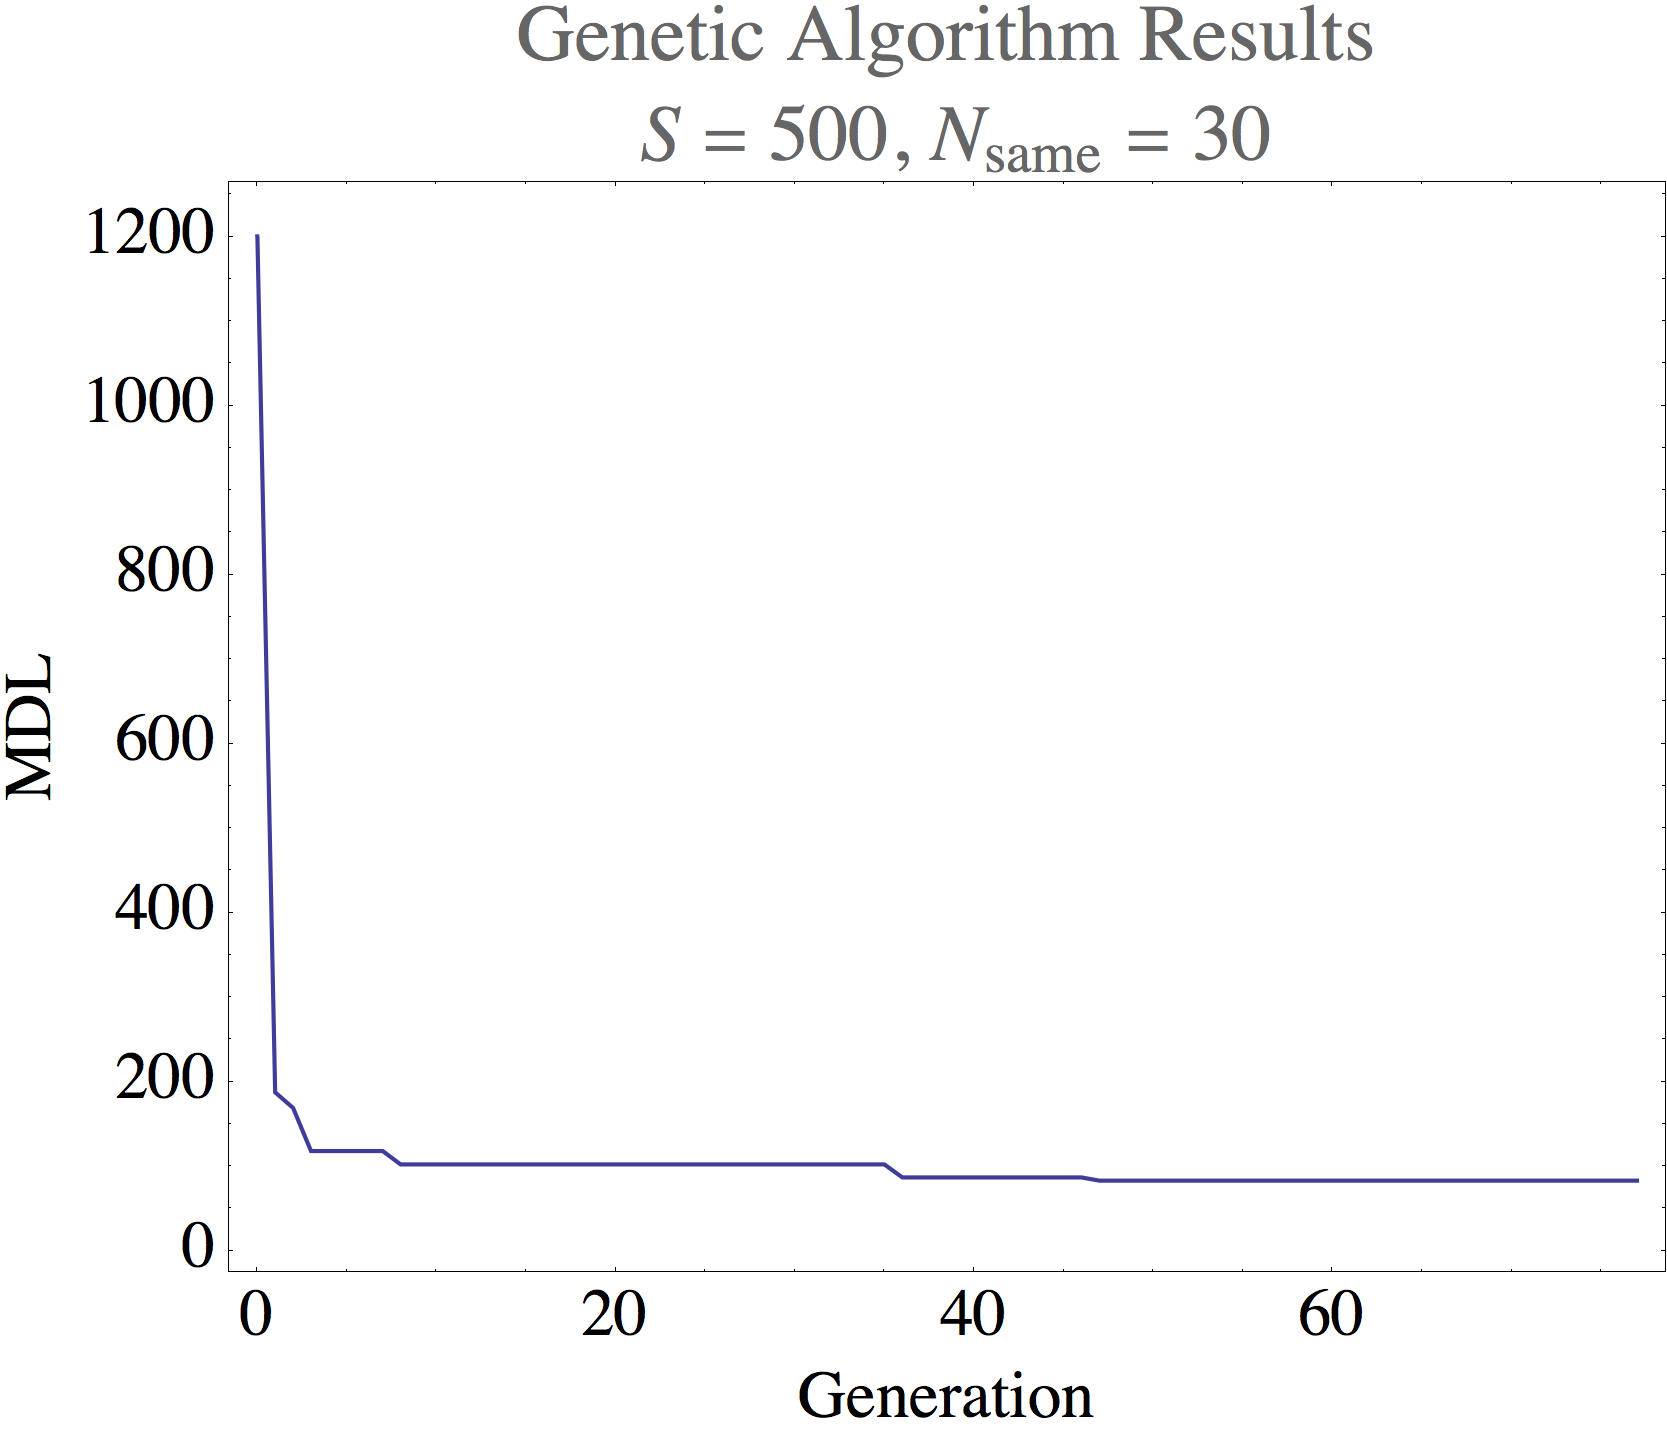
\includegraphics[width=\linewidth,height=0.20\textheight]{mdl_gen_data_500_30.png}\\\hline
      AIC&
      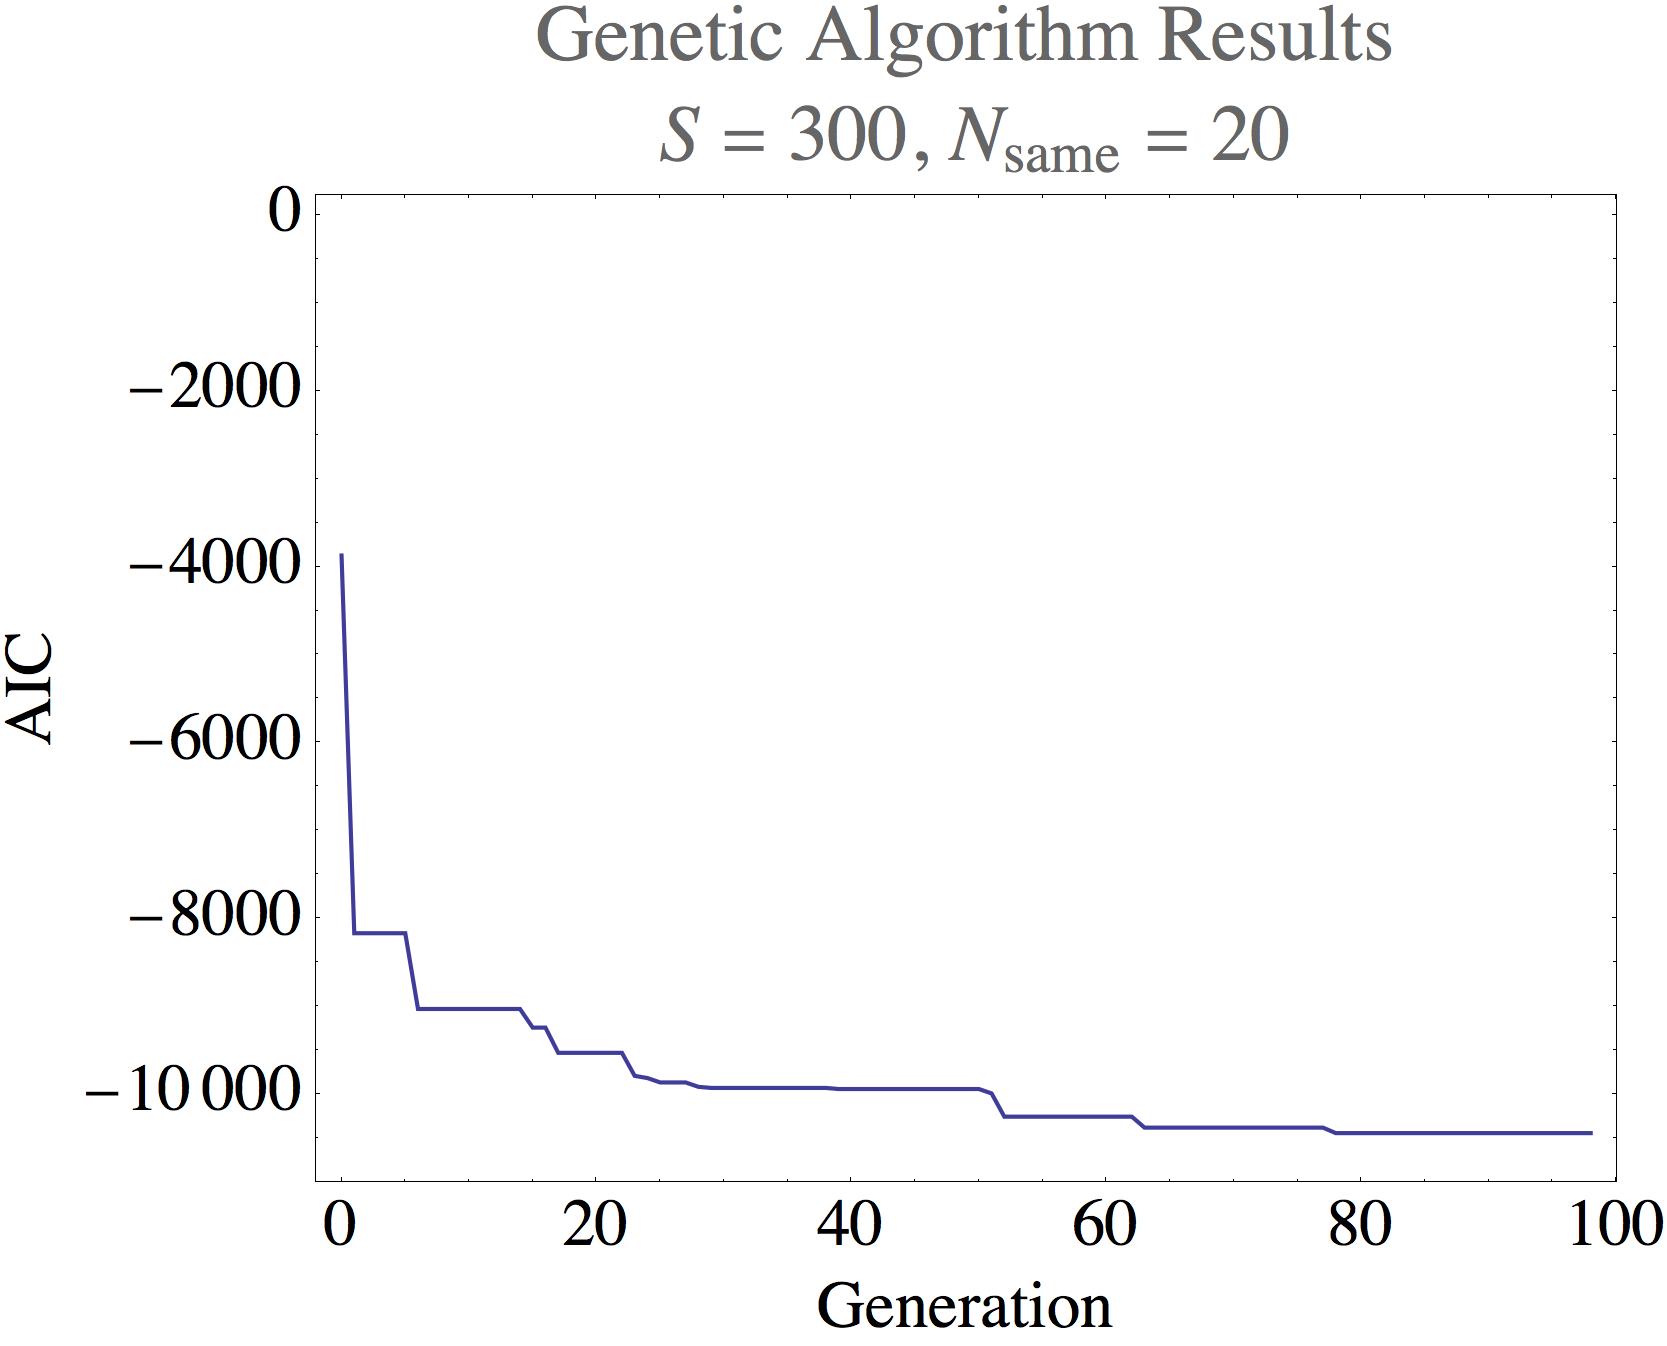
\includegraphics[width=\linewidth,height=0.20\textheight]{aic_gen_data_300_20.png}&
      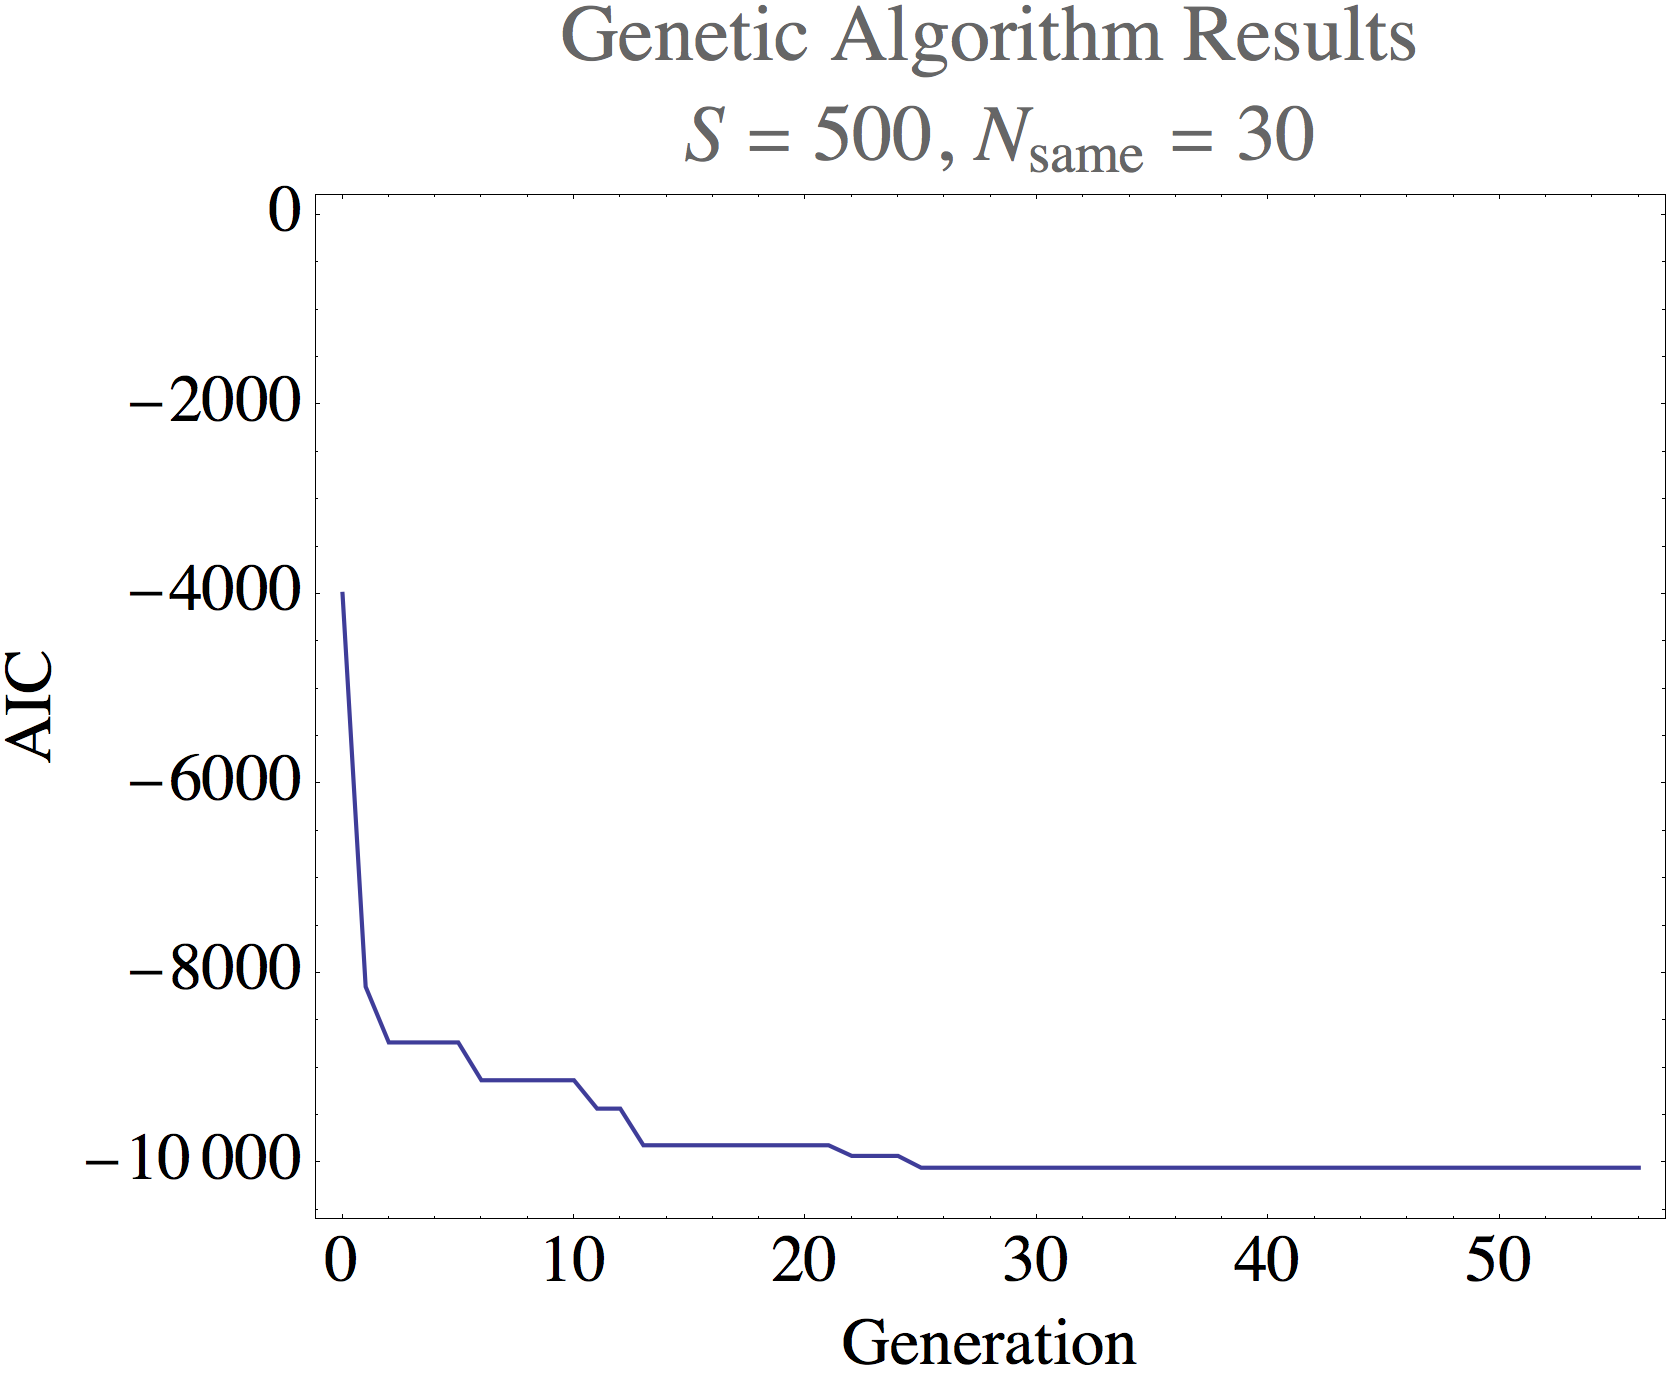
\includegraphics[width=\linewidth,height=0.20\textheight]{aic_gen_data_500_30.png}\\\hline
    \end{tabular}
  \end{center}
\end{table*}

\begin{table*}[h]
  \begin{center}
    \renewcommand{\arraystretch}{1.5}
    \begin{tabular}{| >{\centering\arraybackslash}m{0.5in} |  >{\centering\arraybackslash}m{2.5in} |  >{\centering\arraybackslash}m{2.5in} | }
      \hline
      &$S=300,N_{\textrm{stop}}=20$&$S=500,N_{\textrm{stop}}=30$\\\hline
      MDL&
      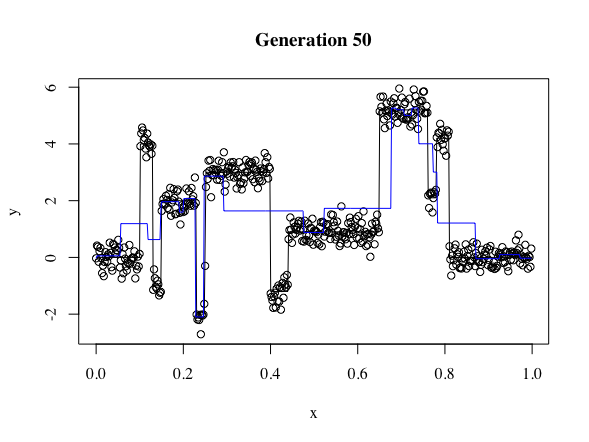
\includegraphics[width=\linewidth,height=0.20\textheight]{mdl_results_300_20.png}&
      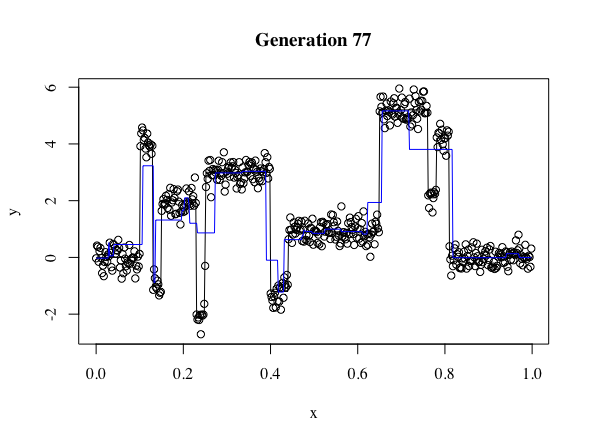
\includegraphics[width=\linewidth,height=0.20\textheight]{mdl_results_500_30.png}\\\hline
      AIC&
      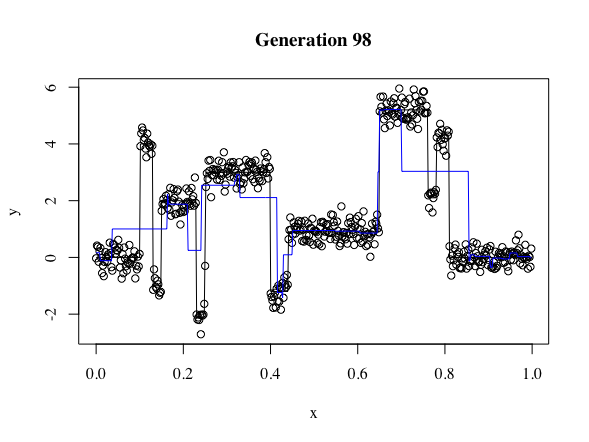
\includegraphics[width=\linewidth,height=0.20\textheight]{aic_results_300_20.png}&
      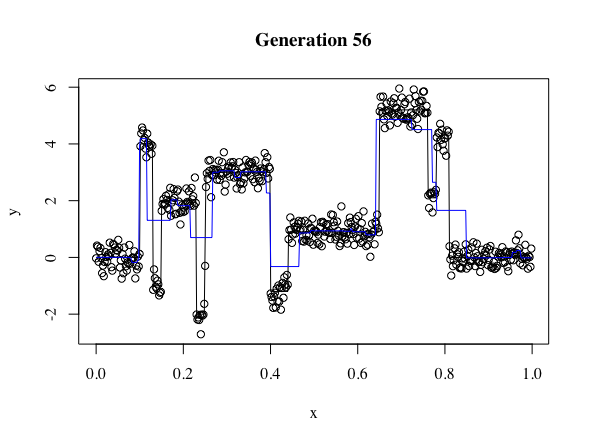
\includegraphics[width=\linewidth,height=0.20\textheight]{aic_results_500_30.png}\\\hline
    \end{tabular}
  \end{center}
\end{table*}

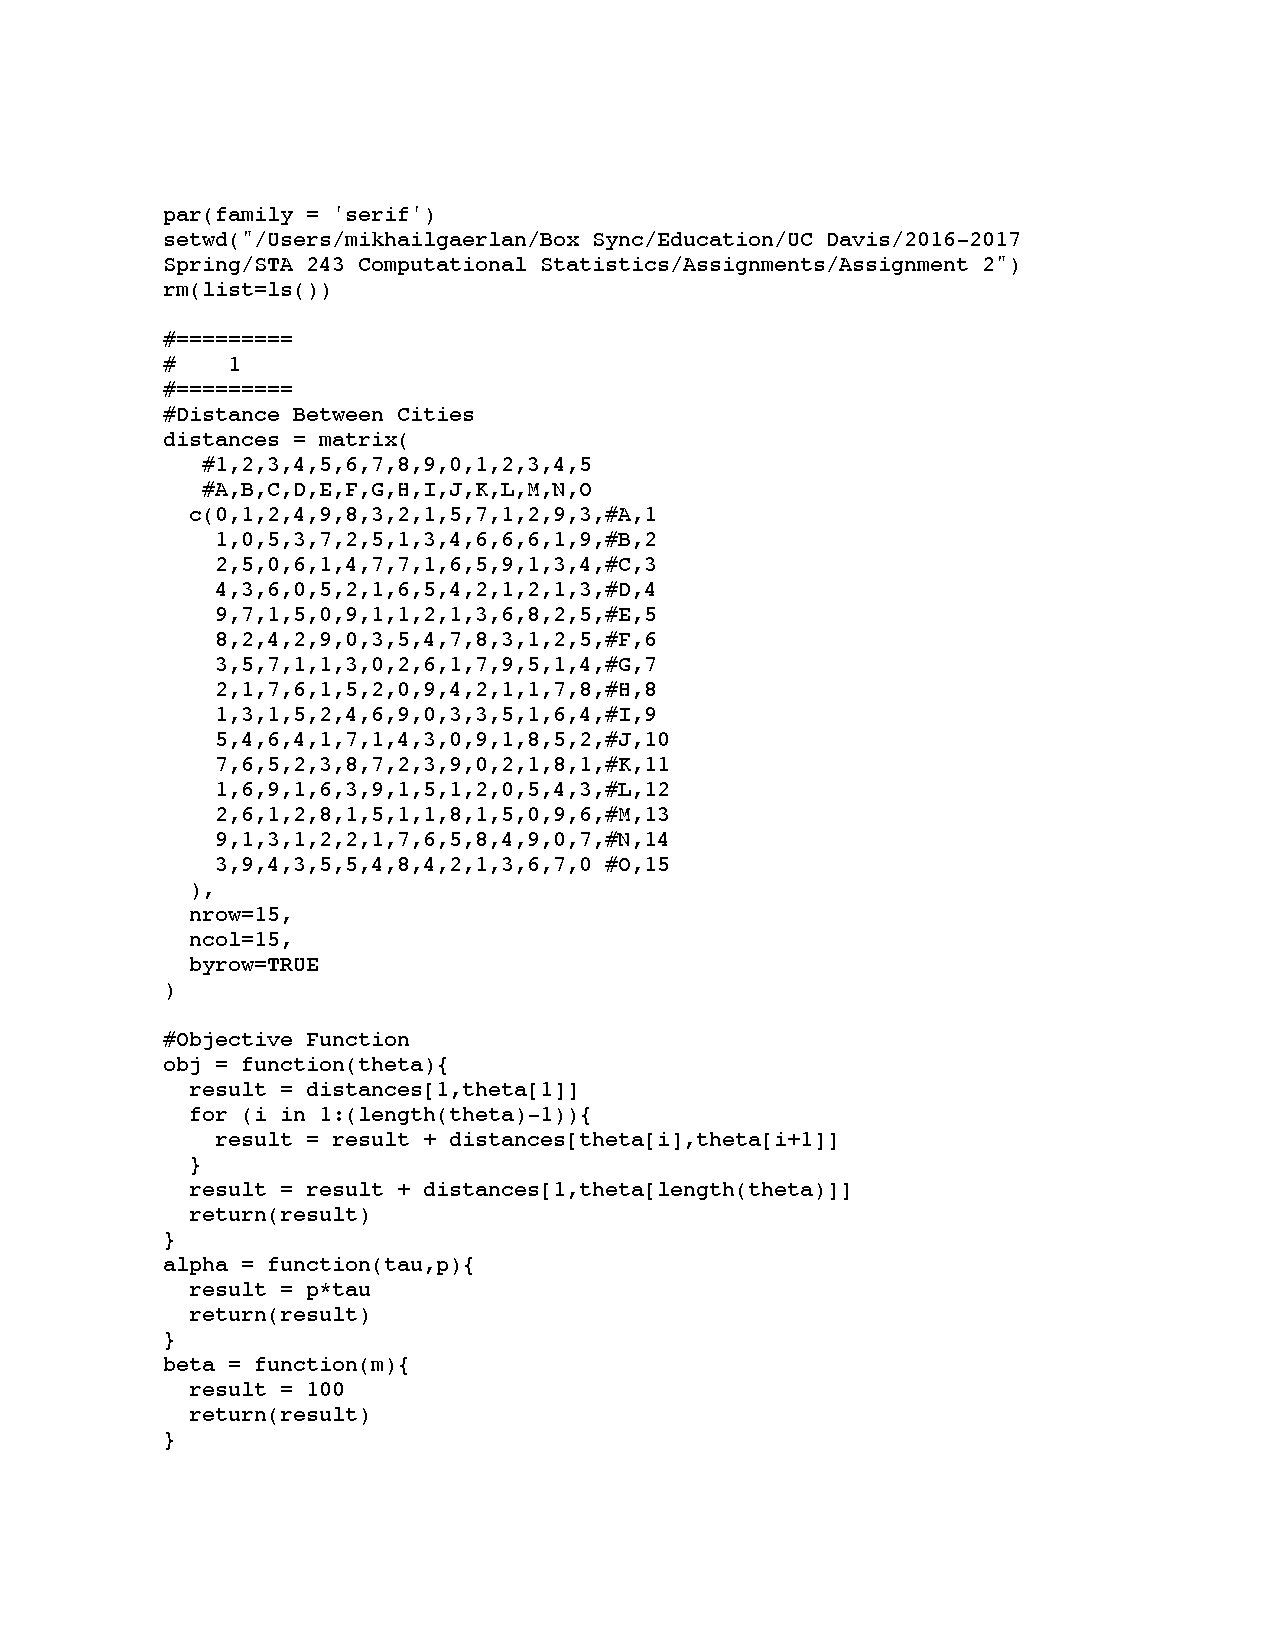
\includepdf[pages={1-3}]{simanneal.pdf}
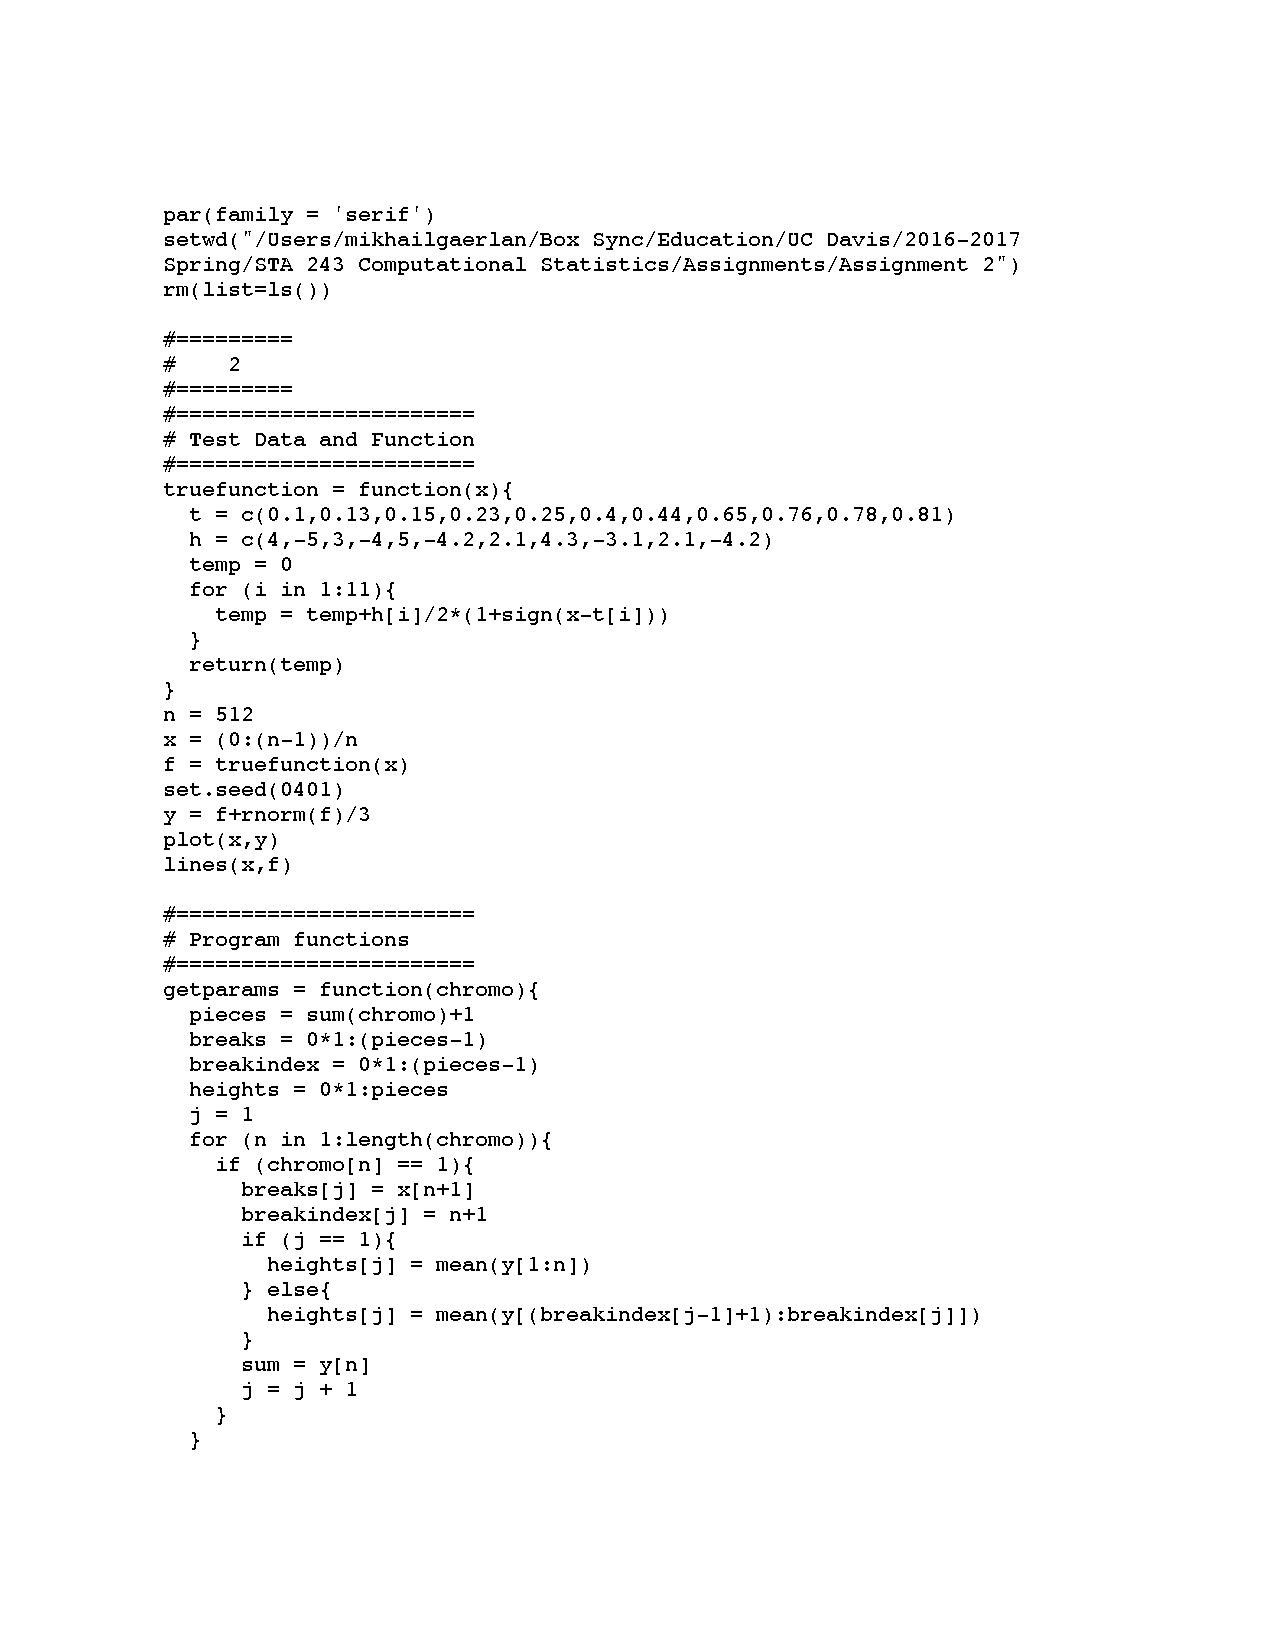
\includepdf[pages={1-7}]{genalg.pdf}

\end{document}